%
% $Id: $
%
%
% Compilar a .pdf con LaTeX (pdflatex)
% Es necesario instalar Beamer (paquete latex-beamer en Debian)
%

%
% Gráficos:
% Los gráficos pueden suministrarse en PNG, JPG, TIF, PDF, MPS
% Los EPS deben convertirse a PDF (usar epstopdf)
%

\documentclass{beamer}
\usetheme{Warsaw}
\usebackgroundtemplate{
\includegraphics[width=\paperwidth]{format/libresoft-bg-soft.png}}
\usepackage[spanish]{babel}
\usepackage[utf8]{inputenc}
\usepackage{graphics}
\usepackage{amssymb} % Simbolos matematicos

%\definecolor{libresoftgreen}{RGB}{162,190,43}
%\definecolor{libresoftblue}{RGB}{0,98,143}

%\setbeamercolor{titlelike}{bg=libresoftgreen}

%% Metadatos del PDF.
\hypersetup{
  pdftitle={Economic Aspects of Libre Software / Master on Libre Software (URJC)},
  pdfauthor={Jesus M. Gonzalez-Barahona, Felipe Ortega},
  pdfcreator={GSyC/LibreSoft, Universidad Rey Juan Carlos},
  pdfproducer=PDFLaTeX,
  pdfsubject={},
}
%%

%\includeonly{presentation}
%\includeonly{introduction}
%\includeonly{economic-impact}
%\includeonly{oss-business-models}
\includeonly{innovation}
%\includeonly{sustainability}
% \includeonly{control-steering-mechanisms}
% \includeonly{rejuvenetion-community-floss}
% \includeonly{single-vendor-community-floss}
%\includeonly{oracle-sun-case-study}

%\includeonly{oss-business-models-statements}
%\includeonly{questions-video-leadbeater}
%\includeonly{oss-business-models-exercise, open-core-debate, build-oss-business-model}

\AtBeginSection[]
{
\begin{frame}<beamer>
\begin{center}
{\Huge \insertsection}
\end{center}
\end{frame}
}

\begin{document}

\title{Economic Aspects of Libre Software }
\subtitle{Master on Libre Software (URJC) \\
\url{http://master.libresoft.es}}
\author{Jesus M. Gonzalez-Barahona, Felipe Ortega}
\institute{jgb@gsyc.es jfelipe@libresoft.es\\
@jgbarah @felipe
GSyC/LibreSoft, Universidad Rey Juan Carlos}

\date{November 2011}

\frame{
\maketitle
\begin{center}

\includegraphics[width=6cm]{format/gsyc-urjc}
\end{center}
}


% Si el titulo o el autor se quieren acortar para los pies de página
% se pueden redefinir aquí:
%\title{Titulo corto}
%\author{Autores abreviado}


%% LICENCIA DE REDISTRIBUCION DE LAS TRANSPAS
\frame{
~
\vspace{3cm}

\begin{flushright}
\copyright 2010, 2011 Jesus M. Gonzalez-Barahona, Felipe Ortega. \\

Some rights reserved. \\
This document is distributed under the \\
Creative Commons Attribution-ShareAlike 3.0 licence, \\
available in \\
\url{http://creativecommons.org/licenses/by-sa/3.0}

The original version of this document is available at \\
\url{http://master.libresoft.es}
\end{flushright}
}
% Slides

%% presentation.tex
%%
%% Presentation of the course ``Master Thesis" of the Official Master on Libre Software (URJC)
%% http://master.libresoft.es
%%

%%---------------------------------------------------------------------
%%---------------------------------------------------------------------

\section{Presentation of the Master Thesis Course}

%%---------------------------------------------------------------

\begin{frame}
\frametitle{Administrative data}

\begin{itemize}
\item Both semesters, 12 ECTS credits
\item Teachers:
  \begin{itemize}
  \item Gregorio Robles (grex at gsyc.urjc.es)
  \item Jesus M. Gonzalez-Barahona (jgb at gsyc.urjc.es)
  \item Departamento de Sistemas Telem�ticos y Computaci�n (GSyC)
  \item Rooms 109 and 120 Departamental II (M�stoles campus)
  \item Room 103 Biblioteca (Fuenlabrada campus)
  \end{itemize}
\item Schedule: see Calendar
\item Sessions:
  \begin{itemize}
  \item Classroom 215, Aulario II, Fuenlabrada campus
  \end{itemize}
\item Moodle course (please, join it as soon as possible): \\
  \url{http://docencia.etsit.urjc.es/moodle/course/view.php?id=134}
\end{itemize}
\end{frame}

%%---------------------------------------------------------------

\begin{frame}
\frametitle{Goals}

Primary Goal: 
To apply the lessons and practices learned in this master
to a real problem

Secondary goal
To do it in one term

\end{frame}

%%---------------------------------------------------------------


\begin{frame}
\frametitle{Evaluation}

\begin{itemize}
\item 
\end{itemize}

\end{frame}

%%---------------------------------------------------------------

\begin{frame}
\frametitle{}

\begin{itemize}
\item 
\end{itemize}

\end{frame}

%%---------------------------------------------------------------

\begin{frame}
\frametitle{}

\begin{itemize}
\item 
\end{itemize}

\end{frame}

%%---------------------------------------------------------------

\begin{frame}
\frametitle{}

\begin{itemize}
\item 
\end{itemize}

\end{frame}


%%---------------------------------------------------------------

\begin{frame}
\frametitle{Some references}

\begin{itemize}
\item  \\
  \url{}
\item Introduction to libre software (book) \\
  \url{http://curso-sobre.berlios.de/introsobre}
\end{itemize}

\end{frame}

%% introduction.tex
%%
%% Introduction to the course ``Economic aspects'' of the
%%   Official Master on Libre Software (URJC)
%%   http://master.libresoft.es

%%---------------------------------------------------------------------
%%---------------------------------------------------------------------
\section{Introduction and motivation}

%%---------------------------------------------------------------

\begin{frame}
\frametitle{The growth of libre software (1)}

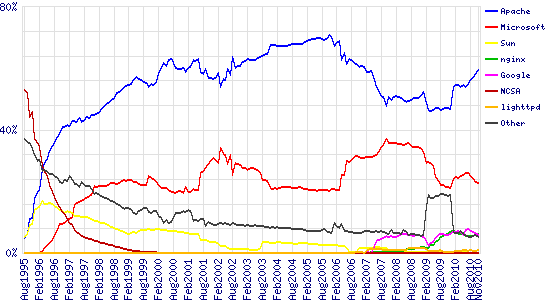
\includegraphics[height=6cm]{webservers-share-2010-11}

\begin{flushright}
Netcraft Survey, November 2010 \\
{\small \url{http://news.netcraft.com/archives/2010/11/05/november-2010-web-server-survey.html}}
\end{flushright}
\end{frame}

%%---------------------------------------------------------------

\begin{frame}
\frametitle{The growth of libre software (2)}

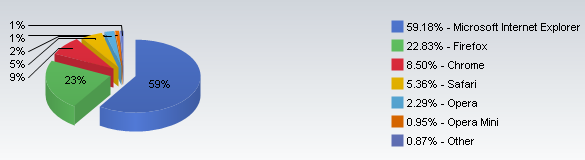
\includegraphics[height=3.5cm]{webbrowsers-share-2010-10}

\begin{flushright}
Net Market Share Report, October 2010 \\
{\small \url{http://www.netmarketshare.com/}}
\end{flushright}
\end{frame}

%%---------------------------------------------------------------

\begin{frame}
\frametitle{The growth of libre software (3)}

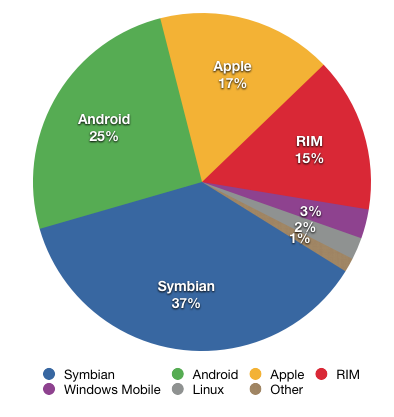
\includegraphics[height=5cm]{smartphone-share-gartner-2010-q3}

\begin{flushright}
Competitive Landscape: Mobile Devices, 3Q10 (Gartner)\\
Worldwide smartphone sales, 3rd Q 2010 \\
{\small \url{http://www.gartner.com/it/page.jsp?id=1466313}} \\
(graph from Wikimedia Commons)
\end{flushright}
\end{frame}


%%---------------------------------------------------------------

\begin{frame}
\frametitle{The adoption of libre software (1)}

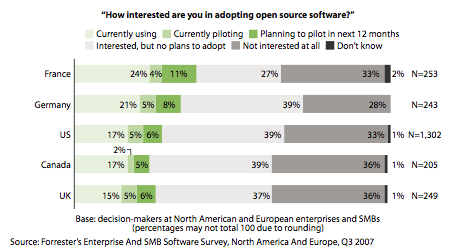
\includegraphics[height=5cm]{adoption-interest-forrester-2007-q3}

\begin{flushright}
Open Source Adoption: Notes From The Field \\
(Forrester, July 2008) \\
{\small \url{http://www.forrester.com/rb/Research/open_source_adoption_notes_from_field/q/id/46279/t/2}} 
\end{flushright}
\end{frame}

%%---------------------------------------------------------------

\begin{frame}
\frametitle{The adoption of libre software (2)}

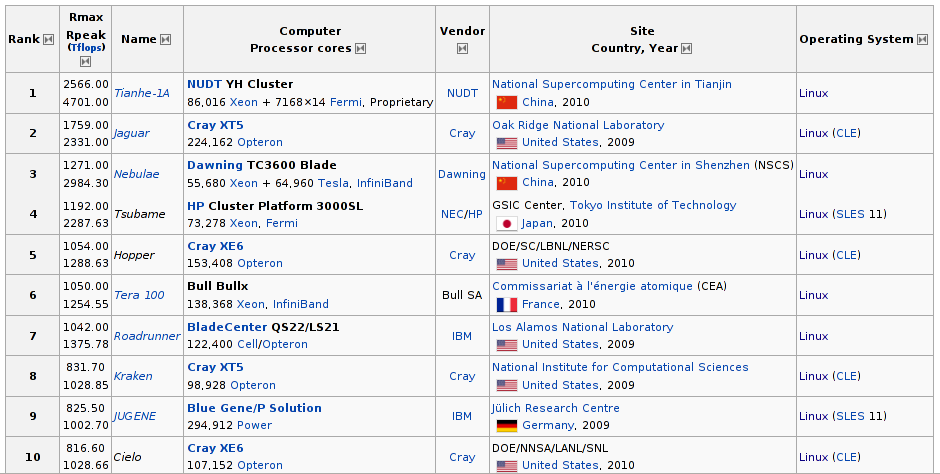
\includegraphics[height=6cm]{top-10-supercomputers-2010-11}

\begin{flushright}
36th TOP500 List (November 2010) \\
{\small \url{http://www.top500.org} \url{http://en.wikipedia.org/wiki/TOP500}} 
\end{flushright}
\end{frame}

%%---------------------------------------------------------------

\begin{frame}
\frametitle{The adoption of libre software (3)}

\begin{center}
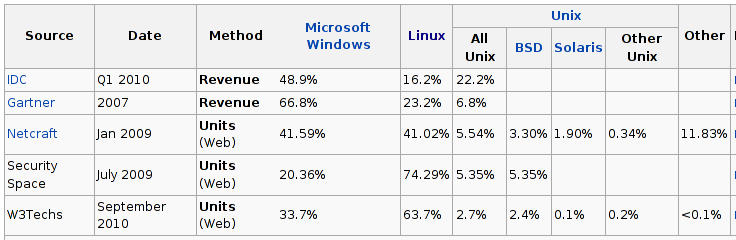
\includegraphics[height=4cm]{server-os-share-2010}
\end{center}

\begin{flushright}
Server market share, operating systems (Wikipedia) \\
{\footnotesize \url{http://en.wikipedia.org/wiki/Usage_share_of_operating_systems}} 
\end{flushright}
\end{frame}

%%---------------------------------------------------------------

\begin{frame}
\frametitle{The adoption of libre software (4)}

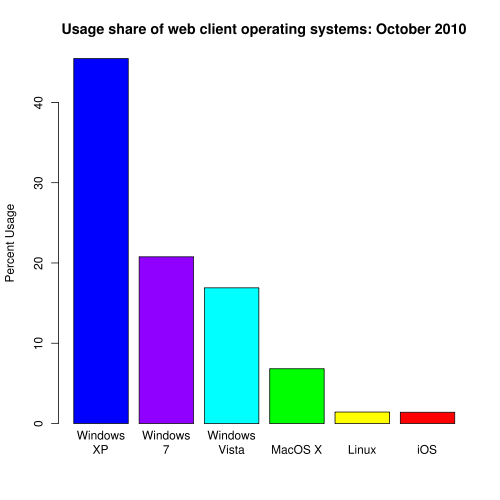
\includegraphics[height=6cm]{desktop-os-marketshare-2010-10}

\begin{flushright}
Usage share of web client operating systems \\
(Wikipedia, October 2010, median of usage studies) \\
{\small \url{http://en.wikipedia.org/wiki/Usage_share_of_desktop_operating_systems}} 
\end{flushright}
\end{frame}

\end{frame}




\section{Economic impact}

%%---------------------------------------------------------------

\begin{frame}
\frametitle{The (business, economic) role of libre software}

\begin{itemize}
\item Functionality: \\
  Easy access to cutting-edge functionality
\item Acquisition of technology: \\
  Libre software is a transfer of technology engine
\item Economic efficiency: \\
  In many cases, libre software case is the most efficient
\item New opportunities: \\
  Libre software changes rules and permits new opportunities
\item Service economy: \\
  Software as a service, instead of software as a product
\item Adaptability, conformance to needs: \\
  Any change is possible
\item Impact: \\
  Free distribution facilitates a massive impact
\end{itemize}
\end{frame}

%%---------------------------------------------------------------

\begin{frame}
\frametitle{Specific impact in the business fabric}

\begin{itemize}
\item Creation of production fabric: \\
  Expenditure in services, network of companies of different sizes
\item Creation of quality employment: \\
  Jobs related to development, maintenance, management, innovation
\item Cost savings, better use of public expenditure (funds for development):
  More and better impact of public expenditure
\item Improved competitiveness: \\
  Use of specific libre software, incremental development in IT sectors
\item Promotion of the value of innovation: \\
  Common base, added value provided by innovation
\end{itemize}

\end{frame}

%%---------------------------------------------------------------

\begin{frame}
\frametitle{Libre software as a disruptive factor}

\begin{center}
{\LARGE
Libre software means new opportunities \\
with disruptive potentials, \\
creation of a sustainable production fabric \\
and provision of means for improvements in many sectors
}
\end{center}

\end{frame}

%%---------------------------------------------------------------

\begin{frame}
\frametitle{Some consequences of software ``freedom''}

\begin{itemize}
\item \textbf{Cost}: model very different from proprietary software
\item \textbf{Openness}: can be modified, inspected, studied
\item \textbf{Distribution}: new channels, new methods
\item \textbf{Development}: `surprising' development models
\item \textbf{Maintenance and support}: Real competition
\end{itemize}

Mixture of two powerful mechanisms:

\begin{itemize}
\item Competition (with the same software base)
\item Cooperation (even involuntary)
\end{itemize}

\end{frame}

%%---------------------------------------------------------------

\begin{frame}
\frametitle{Some business arguments}

\begin{itemize}
\item Advantages of public scrutiny and chances for improvements
\item Real competition in development and  maintenance
\item Technical feasibility vs. marketing
\item Easy testing, deployment, update
\item Lower barriers to business opportunities
\item Non-formal collaboration and pooling of resources
\item Technology transfer
\item Libre software as an strategic tool
\end{itemize}

\end{frame}


%%---------------------------------------------------------------

\begin{frame}
\frametitle{What disappears when a business uses libre software?}

\begin{itemize}
\item Dependence on monopolies: \\
  Real competition, better products, better services
\item Importance of vendor reliability: \\
  Future depends on product acceptance
\item Decisions taken based on few elements: \\
  Software can be tested in its real environment, at a very low cost
\item Dependence on the strategy of providers: \\
  Decisions on the evolution of a product taken for those contributing with resources
\item Confidence on ``black boxes'': \\
  Software can be studied in detail
\end{itemize}
\end{frame}

%%---------------------------------------------------------------

\begin{frame}
\frametitle{Conclusions?}

\begin{itemize}
\item Libre software is a viable business option
\item Allows for new business opportunities...
\item ...but it is important to know how to take advantage of those
\end{itemize}

\end{frame}






%%

\section{FLOSS business models}

\subsection{Introduction}

\begin{frame}
\frametitle{The million dollar question}

Once upon a time, the key question for companies/projects/individuals entering the
FLOSS universe was:

\begin{itemize}
 \item \textit{How can we make money with FLOSS?}
\end{itemize}

\pause
But now, the question is

\begin{itemize}
\item \textit{Which are the most successful business strategies that we can adopt around FLOSS?}
\end{itemize}
\end{frame}

\begin{frame}
 \frametitle{Origin: open innovation}
 \begin{itemize}
  \item Some (few) people are still against the added-value provided by knowledge aperture (source
code is just an example).
  \item Case study: \textbf{GoldCorp} \texttt{http://www.goldcorp.com/}
    \begin{itemize}
    \item Traditional mining company, gold business, needs to find new veins.
    \item Executive President Rob McEwen publishes open contest (2000): 575K\$ for participants
    who offer best methods to choose new extraction points.
    \item 80\% of answers produced positive results.
    \item 100\$ invested in 1993 is worth over 3.000\$ in 2005.
    \end{itemize}
  \item However, \textbf{crowdsourcing is orthogonal to libre software}
 \end{itemize}
\end{frame}

\begin{frame}
 \frametitle{Current trends}
 \begin{itemize}
 \item ``\textit{There is no silver bullet}''
 \item Every company/project/individual should select appropriate strategies for their particular needs.
 \item And being alert to change/evolve their model on the fly, in response to rapid changes in the market
and surrounding conditions.
 \item Luckly, there exist \textbf{many} options to choose from.
 \end{itemize}
\end{frame}

\begin{frame}
 \frametitle{False myths}
\begin{itemize}
 \item Many companies justify the cost of proprietary software with the economic cost of production (development) process.
\item Two types of product value:
    \begin{itemize}
     \item \alert{Use} value: Economic value as a tool, productivity growth (value as an intermediate good).
     \item \alert{Sale} value: Value as a market product (value as a final product).
    \end{itemize}
\item Aprox. 75\% of salaried programmers work is devoted to
\alert{maintenance} tasks, not to \alert{development} of new features.
\end{itemize}

\end{frame}

\begin{frame}
 \frametitle{False myths}
\begin{itemize}
 \item Contrary to other products, the true \alert{value} of software does not lie in its production
or replacement cost (food, cars, engines, appliances...).
 \item The upper limit of the value of software for clients is imposed by the expected value of the future service
that sellers offer to clients.
      \begin{itemize}
       \item Software stability.
       \item Help-desk, support services.
       \item Documentation.
       \item Software customization.
       \item Training and certification.
      \end{itemize}
  \pause
  \centering{\alert{services == source of revenues}}
\end{itemize}

\end{frame}

\begin{frame}
 \frametitle{False myths}
\begin{itemize}
 \item The organizational model of libre software allows to provide services in a more profitable,
scalable and sustainable way.
\begin{itemize}
 \item \alert{Users} become \alert{clients}.
 \item \alert{Scalability} in failures identification and solution.
 \item \alert{Sharing risks} and production \alert{costs}.
 \item Monopolistic practices made \alert{difficult}.
\end{itemize}
\end{itemize}

\end{frame}

\begin{frame}
 \frametitle{False myths}
\begin{itemize}
 \item Myth: ``The Commons tragedy''.
 \item Any business model would be doomed to fail, or else, to result 
in a new scenario with closed solutions.
 \item Antidote: In fact \alert{software use} does not \alert{reduce} but it
\alert{grows its value}.
    \begin{itemize}
    \item Larger user community (potential clients).
    \item Benefit from patches and proposed solutions.
    \item Benefit from new features.
    \item Contributing to leverage product quality (guarantee absence of conflicts 
with business interests).
    \end{itemize}
\centering{\alert{``Inverse commons''}}
\end{itemize}
\end{frame}

\begin{frame}
 \frametitle{Central idea}
\Large{The \alert{business model} must always pivot on the \alert{use value}, not on the
sale value.}
\end{frame}

\subsection{Taxonomy of FLOSS business models}

%\subsection{FLOSS: A guide for SMEs}

\begin{frame}
 \frametitle{FLOSS: A guide for SMEs}
\begin{center}
 \begin{LARGE} FLOSS by itself is not, and it has never been, a business model. \end{LARGE}
\end{center}
\begin{center}
 Companies must desing a \alert{strategy}, create a \alert{business plan} and ensure 
\alert{securing benefits} aimed to a sustainable growth.
\end{center}
\begin{center}
 FLOSS can improve \alert{viability} and \alert{efficiency} of many business models.
\end{center}


\end{frame}

\begin{frame}
 \frametitle{FLOSS: A guide for SMEs}
 \begin{itemize}
  \item Report ellaborated for FLOSSMETRICS, EU FP6 project.
  \item Analysis of 218 companies receiving at least 25\% of their total revenues directly or indirectly from FLOSS.
  \item Identifying common business strategies around FLOSS.
  \item Recommendations about required conditions to apply each model.
 \end{itemize}
\end{frame}

\begin{frame}
 \frametitle{3 axes influencing software landscape}
 \begin{itemize}
  \item \alert{Software model}
  \begin{itemize}
   \item Proprietary vs. libre software.
  \end{itemize}
  \item \alert{Development model}.
  \begin{itemize}
   \item Barriers to collaboration.
   \item Single developer/reduced group vs. large community, global outreach.
  \end{itemize}
  \item \alert{Business model}.
  \begin{itemize}
   \item Type of revenues model.
   \item Numerous options: Training, support, on-demand changes, productizing, SaaS, etc.
  \end{itemize}
 \end{itemize}
\end{frame}

\begin{frame}
 \frametitle{Strategic uses of libre software}
 \begin{itemize}
  \item The Gartner consulting group pointed out: in 2012, use of libre software would reach 90\% of companies worldwide.
  \item Companies forced to adapt their software to work under multiple conditions.
  \item Emerging trend in big companies towards source code release under FLOSS licenses.
More active interaction with nearby projects.
  \item Proprietary software success is now guaranteed only if there are no alternative and reliable FLOSS options.
 \end{itemize}
\end{frame}


\begin{frame}
 \frametitle{Carlo Daffara taxonomy (FLOSSMETRICS)}
 \begin{itemize}
  \item \textit{Dual licensing}: FLOSS version and proprietary version.
  \item \textit{Open core}: Allows mixing FLOSS and proprietary elements.
  \item \textit{Product specialists}: Superior knowledge, additional services.
  \item \textit{Platform providers}: Integration, product testing.
  \item \textit{Aggregate support providers}: Primer nivel de soporte para diferentes
tipos de software libre.
  \end{itemize}
  \end{frame}
  
  \begin{frame}
 \frametitle{Carlo Daffara taxonomy (FLOSSMETRICS)}
 \begin{itemize}
\item \textit{Selection/consulting companies}: Closer to the analyst role, minimum impact on FLOSS communities.
  \item \textit{Legal certification and consulting}: Assessment on license compatibility.
  \item \textit{Training and documentation}: Either as part of a broader support contract or companies exclusively devoted
to this market area.
  \item \textit{R\&D cost sharing}: Initial investment + leveraging community to reduce R\&D costs.
  \item \textit{Indirect revenues}: Baseline for sales of associated products or services (commodities).
 \end{itemize}
\end{frame}

\begin{frame}
\frametitle{Distribution of models identified in the study}
\begin{center}
\begin{figure}
 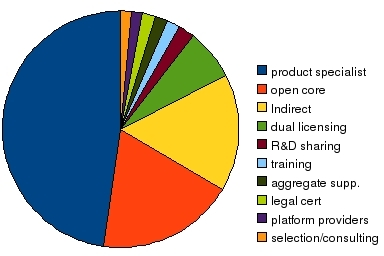
\includegraphics[height=4.5cm]{figs/models-share.jpg}
 \caption{\small Taken from ``FLOSS: A guide for SMEs''. C. Daffara (FLOSSMETRICS EU FP6)}
\end{figure}
\begin{figure}
 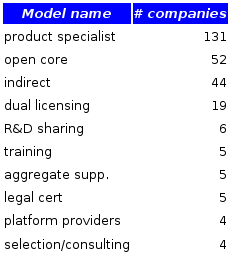
\includegraphics[height=4.5cm]{figs/models-share-numbers.png}
\end{figure}
\end{center}
\end{frame}

\begin{frame}
\frametitle{Evolution CAGR in FLOSS business}
\begin{center}
\begin{figure}
 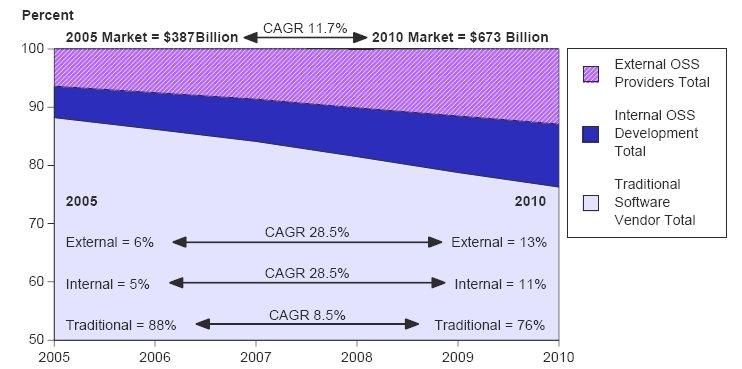
\includegraphics[height=4.5cm]{figs/Economic-Gartner.jpg}
 \caption{\small Taken from ``Open Source going mainstream'', Gartner group report.}
\end{figure}
\end{center}
\end{frame}

\begin{frame}
\frametitle{Companies running business around FLOSS (selection)}
\begin{center}
\begin{figure}
 
\includegraphics[height=4.5cm]{figs/floss-companies.jpg}
 \caption{\small Taken from ``FLOSS: A guide for SMEs'', Carlo Daffara (FLOSSMETRICS EU FP6)}
\end{figure}
\end{center}
\end{frame}



% \subsection{Clasificación extendida}
% \begin{frame}
%  \frametitle{Alternativas de modelos de negocio (extendida)}
%  \begin{itemize}
%   \item Con financiación externa
%   \begin{itemize}
%    \item El fundador generalmente decide cómo y dónde gastar los recursos.
%    \item Orientado hacia la producción de software.
%    \item En cierto modo, es una estrategia de esponsorización.
%   \end{itemize}
%   \item Auto-financiados
%   \begin{itemize}
%    \item Ingresos de las actividades de la compañía.
%    \item Puede haber desarrollo de software o no.
%   \end{itemize}
%   \item Desarrollado sin financiación directa.
%   \item Desarrollado para uso interno.
%   \item Modelos mixtos.
%  \end{itemize}
% \end{frame}
% 
% \begin{frame}
%  \frametitle{Financiación externa}
%  \textbf{Financiación pública}
%  \begin{itemize}
%   \item Similar a proyectos de I+D.
%   \item Financiación puede venir de instituciones que promuevan I+D.
%   \item Institución financiadora normalmente no busca beneficios directos.
%   \item Expresamente realizada sólo en casos particulares; principalmente como 
% ``subproducto`` de un contrato.
%  \end{itemize}
% \end{frame}
% 
% \begin{frame}
%  \frametitle{Negocios con financiación externa}
%  \textbf{Financiación externa (motivaciones y casos de estudio)}
%  \begin{itemize}
%   \item ``Científica'': Software requerido para producir resultados
% que deben estar disponibles, para publicación científica.
%   \item ``Pre-competitive'': Beneficios industriales de resultados pre-competitivos.
%   \item ``Promoción de estandar'': Implementación de referencia o estándar (probablemente, la
% norma o estándar también abierta).
%   \item `Motivación social'': Financiación de infraestructura básica para la Sociedad de la Información.
%   \item  Caso de estudio: Gnat (compilador de Ada), alrededor de 1 M\$ del Gobierno Federal EE.UU.
% a la NYU para su desarrollo.
%   \end{itemize}
% \end{frame}
% 
% \begin{frame}
%  \frametitle{Negocios con financiación externa}
%  \textbf{Fianciación privada sin ánimo de lucro}
%  \begin{itemize}
%   \item Normalmente, proviene de de ONGs y fundaciones privadas.
%   \item Motivación ``directa'': Producción de software libre.
%   \item Motivación ``indirecta'': Contribuye a resolver el problema de creación de solución software.
%   \item En general, mecanismos similares a la financiación pública.
%   \item Casos de estudio:
%   \begin{itemize}
%    \item Free Software Foundation
%    \item Open Bioinformatics Foundation
%   \end{itemize}
%  \end{itemize}
%  \hfill \large \texttt{http://fsf.org}\\
%  \hfill \large \texttt{http://open-bio.org}
% \end{frame}
% 
% \begin{frame}
%  \frametitle{Negocios con financiación externa}
%  \textbf{Financiación de fuentes interesadas en mejoras}
%  \begin{itemize}
%   \item Alguien necesita mejoras en un producto de sofware libre.
%   \item Desarrollo financiado por un grupo o compañía.
%   \item Caso de estudio:
%   \begin{itemize}
%    \item Corel quería tener una versión de sus productos para GNU/Linux.
%    \item Wine podía contribuir a ahorrar costes si se mejoraba.
%    \item Corel financió contribuciones de Macadian para Wine, incluyendo las que
% ellos mismos necesitaban.
%   \end{itemize}
%   \hfill \large \texttt{http://www.macadamian.com/news/wine.html}
%  \end{itemize}
% \end{frame}
% 
% \begin{frame}
%  \frametitle{Negocios con financiación externa}
%  \textbf{Financiación indirecta}
%  \begin{itemize}
%   \item Financiación de desarrollo de software a través de beneficios obtenidos mediante productos
% relacionados.
%   \item Normalmente, las ventajas (incluyendo aquellas que se ponen a la venta) no son exclusivas.
%   \item Ventajas mejores cuanto mayor es el porcentaje de mercado en ese nicho.
%   \item Ejemplos: libros, hardware, distribuciones.
%   \begin{itemize}
%    \item O'Reilly financia el desarrollo de Perl development, y es la principal editorial que publica
% sobre este tema.
%    \item RedHat financia desarrollo GNOME para garantizar un escritorio fiable para su propia distribución.
%    \end{itemize}
%  \end{itemize}
%   \hfill \large \texttt{http://oreilly.com}\\
%   \hfill \large \texttt{http://redhat.com}
% \end{frame}
% 
% \begin{frame}
%  \frametitle{Modelos de negocio auto-financiados}
%  \textbf{Basados en un conocimiento superior}
%  \begin{itemize}
%   \item Venta de servicios basada en un mejor conocimiento del producto.
%   \item Conocimiento es principalmente adquirido trabajando en el proyecto y colaborando en su desarrollo.
%   \item Desarrollo del producto también ayuda por motivos de imagen.
%   \item Pero la participación en el desarrollo no es obligatoria.
%   \item Normalmente se vende servicios de consultoría, adaptación, integración, etc.
%  \end{itemize}
% \end{frame}
% 
% \begin{frame}
%  \frametitle{Modelos de negocio auto-financiados}
%  \textbf{Basados en un conocimiento superior pero con limitaciones}
%  \begin{itemize}
%   \item Estos modelos tratan de limitar el efecto de compañías competidoras.
%   \item Típicamente se emplean patentes o licencias propietarias.
%   \item Normalmente, estos mecansimos se aplican en partes pequeñas pero fundamentales del 
% producto desarrollado.
%   \item En la mayoría de casos, la comunidad de software libre desarrolla su propia versión de
% estos componentes.
%  \end{itemize}
% \end{frame}
% 
% \begin{frame}
%  \frametitle{Modelos de negocio auto-finaciados}
%  \textbf{Basados en ser la fuente de un programa}
%  \begin{itemize}
%   \item Similar a aquellos basados en un conocimiento superior.
%   \item Ventaja competitiva obtenida de convertirse en desarrolladores de un
% producto, y tenerlo listo antes que la competencia.
%   \item Muy interesante en términos de imagen.
%   \item Casos de estudio:
%   \begin{itemize}
%    \item Evolution, RedCarpet (Ximian, hoy Novell).
%    \item Zope (Zope Corporation, anteriormente Digital Creations).
%   \end{itemize}
%  \end{itemize}
%  \hfill \large \texttt{http://ximian.com}\\
%  \hfill \large \texttt{http://zope.com}
% \end{frame}
% 
% \begin{frame}
%  \frametitle{Modelos de negocio auto-finaciados}
%  \textbf{Basado en ser la fuente de un programa pero con limitaciones}
%  \begin{itemize}
%   \item Como en el anterior, pero imponiendo algunas limitaciones para excluir a compañías
% competidoras del proceso.
%   \begin{itemize}
%    \item Ejemplo: distribución propietaria durante un tiempo, luego libre
%    \item Ejemplo: distribución limitada durante un tiempo
%   \end{itemize}
%   \item Estos modelos se benefician menos de las ventajas del software libre; al menos desde
% el punto de vista de desarrollo (son menos cooperativos).
%   \item Casos de estudio:
%   \begin{itemize}
%    \item Alladin Ghostscript (un año entre la versión AFPL y la versión GPL).
%    \item Gnat (AdaCore) (versiones en desarrollo sólo para algunos clientes).
%   \end{itemize}
%  \end{itemize}
%  \hfill \large \texttt{http://www.ghostscript.com} 
%  \hfill \large \texttt{http://www.alladin.com}\\
%  \hfill \large \texttt{http://adacore.com}
% \end{frame}
% 
% \begin{frame}
%  \frametitle{Modelos de negocio auto-finaciados}
%  \textbf{Basados en licencias especiales}
%  \begin{itemize}
%   \item Con frecuencia, se basan en la distribución del software bajo dos o más licencias
% diferentes.
%   \item En general, se complementan con labores de consultoría de producto.
%   \item Ejemplos: Distribuciones libres bajo GPL, versiones propietarias para clientes con necesidades
% adicionales/especiales.
%   \item Caso de estudio:
%   \begin{itemize}
%    \item MySQL: \textit{Community} distribuída bajo GPL; \textit{Enterprise}, 
%    versión propietaria directamente soportada por la empresa MySQL AB, con muchas mejoras de valor añadido.
%   \end{itemize}
%  \end{itemize}
%   \hfill \large \texttt{http://mysql.com}
% \end{frame}
% 
% \begin{frame}
%  \frametitle{Modelos de negocio auto-finaciados}
%  \textbf{Basados en la venta de una marca registrada}
%  \begin{itemize}
%   \item Si el nombre gana popularidad, se puede usar para vender casi cualquier cosa.
%   \item Ejemplo: Distribuciones GNU/Linux que venden otros productos/servicios.
%   \item Caso de estudio:
%   \begin{itemize}
%    \item RedHat: Empezó inicialmente vendiendo su distribución, hoy día tiene otros núcleos clave
% de negocio como consultoría, formación, certificación, etc.
%   \end{itemize}
%  \end{itemize}
%  \hfill \large \texttt{http://www.redhat.com}
% \end{frame}
% 
% \begin{frame}
%  \frametitle{Desarrollos sin financiación directa}
%  \begin{itemize}
%   \item La mayoría de los proyectos se desarrollan fundamentalmente de este modo.
%   \item En muchos casos, tenemos ``financiación indirecta'':
%   \begin{itemize}
%    \item Compañías que permiten que sus empleados empleen parte de su tiempo para contribuir
% a software libre.
%    \item Contribuciones de organizaciones que desean cierta funcionalidad.
%    \item Contribución de infraestructuras al proyecto.
%    \item Donaciones.
%   \end{itemize}
%  \end{itemize}
% \end{frame}
% 
% \begin{frame}
%  \frametitle{Desarrollo sin financiación directa}
%   \textbf{Casos de estudio}
%  \begin{itemize}
%   \item Muchos de los grandes proyectos han establecido fundaciones que proporcionan
% cobertura legal y (parcialmente) económica.
%   \begin{itemize}
%    \item Apache Software Foundation
%    \item Gnome Foundation
%    \item KDE e. V.
%    \item Mozilla Foundation.
%    \item Plone Foundation.
%   \end{itemize}
%  \end{itemize}
%   \hfill \large \texttt{http://apache.org}\\
%   \hfill \large \texttt{http://foundation.gnome.org}\\
%   \hfill \large \texttt{http://www.kde.org/areas/kde-ev/}\\
%   \hfill \large \texttt{http://www.mozilla.org/foundation}\\
%   \hfill \large \texttt{http://plone.org/foundation}
% \end{frame}
% 
% \begin{frame}
%  \frametitle{Desarrollos internos}
%  \begin{itemize}
%   \item Al menos en su fase inicial, el producto es sólo para uso interno.
%   \item Los desarrolloadores se benefician del modelo del software libre: contribuciones, informes
% de error, parches, etc.
%   \item Las compañías obtienen beneficios también: continuidad en el soporte, inspección por terceras
% partes, documentación, mayor capacidad de desarrollo etc.
%   \item Si tienen aceptación en el mercado, se pueden comenzar a aplicar otros modelos de negocio.
%   \item Caso de estudio: Cisco Enterprise Print System (CEPS)
%  \end{itemize}
%    \hfill \large \texttt{http://ceps.sourceforge.net}
% \end{frame}
% 
% \begin{frame}
%  \frametitle{Modelos mixtos}
%  \begin{itemize}
%   \item Casi todas las compañías los usan.
%   \item Medidas para fortalecer la imagen de marca.
%   \item Pueden o no contribuir al desarrollo del software.
%   \item En casos raros, estas compañías trabajan exclusivamente con SL.
%   \item Muchas compañías ``tradicionales`` intentan nuevas opciones con el
% software libre.
%   software.
%  \end{itemize}
% \end{frame}
% 
% \subsection{Taxonomía de Hecker}
% \begin{frame}
%  \frametitle{Taxonomía de Frank Hecker (OSI)}
%  \begin{itemize}
%   \item \textit{Soporte de venta}: Venta de servicios relacionados con el producto.
%   \item \textit{Líder de pérdidas}: Venta de otros productos propietarios.
%   \item \textit{Widget frosting}: Promoción de ventas hardware.
%   \item \textit{Accesorización}: Habilitar ventas de productos físicos (libros, etc.).
%   \item \textit{Facilitador de servicios}: Servicios on-line accesibles a través del programa.
%   \item \textit{Véndelo, libéralo}: Versión cíclica del líder de pérdidas.
%   \item \textit{Licencia de marca}: Venta de royalties de marca
%   \item \textit{Franquicia de software}: Franquicia de marca.
%  \end{itemize}
% \end{frame}
% 
% \begin{frame}
%  \frametitle{Recomendaciones para migración de código a software libre}
%  \begin{itemize}
%   \item Compartición de código: Separación clara del código fuente de liberías o módulos que sean
% propietarios.
%   \item Tecnología de terceras partes: Inspeccionar el uso de librerías de terceras partes para evitar
% problemas de licencias.
%   \item Saneamiento de código: Limpieza y preparación de código fuente para contribuciones por parte de
% desarrolladores externos.
%   \item Control de expotación: Consideración de condiciones especiales de exportación de algoritmos criptográficos
% y protocolos y sistemas de seguridad (lista reducida de países fuera de EE.UU.).
%   \item Proceso de desarrollo de producto: Adaptación deprocesos de trabajo internos a nuevas contribuciones.
%  \end{itemize}
% \end{frame}

% %%%%%%%%%%%%%%%%%%%%%%%%%%%%%%%%%%%%%%%%%%%%%%%%%%%%%%%%
% 
\section{Conclusions}

\begin{frame}
 \frametitle{New ways of collaboration}
 \begin{itemize}
  \item Libre software can be adopted as a mean to facilitate new ways of collaboration
among different companies. \textit{Coopetition}.
  \item Several possibilities (collaboration without formal contracts or agreements).
  \item Creating business ecosystems.
  \item Empowering business opportunities.
  \item Inspiration for new applications of information sharing.
 \end{itemize}
\end{frame}

% \begin{frame}
%  \frametitle{Algunos ejemplos interesantes}
%  \begin{itemize}
%   \item AdaCore (antes ACT y ACT Europe).
%   \item Matra Datavision y OpenCascade.
%   \item Sun, StarOffice y OpenOffice.org (ahora Oracle).
%  \end{itemize}
% \hfill \large \texttt{http://www.adacore.com/}\\
% \hfill \large \texttt{http://libre.act-europe.fr/}\\
% \hfill \large \texttt{http://www.opencascade.org/}\\
% \hfill \large \texttt{http://www.opencascade.com/}\\
% \hfill \large \texttt{http://staroffice.com}\\
% \hfill \large \texttt{http://openoffice.org}
% \end{frame}

\begin{frame}
 \frametitle{References}
 \begin{itemize}
  \item ``FLOSS: A guide for SMEs''.
\texttt{http://guide.conecta.it/index.php/Main\_Page}
  \item ``The Magic Cauldron'', Eric Raymond.
  \item ``State of Open Source'', Gartner Group, 2008.
\texttt{http://arstechnica.com/open-source/news/2008/02/}
\texttt{gartner-80-percent-of-commercial-software-}
\texttt{programs-will-include-open-source-by-2012.ars}
  \item The rejuvenetion of community controlled open source.
\texttt{http://blogs.the451group.com/opensource/2009/10/15/}
\texttt{the-rejuvenation-of-community-controlled-open-source/}
 \end{itemize}

\end{frame}

% \begin{frame}
%  \frametitle{Referencias}
%  \begin{itemize}
%   \item ``Free Software, Open Source: Information Society Opportunities
%   for Europe?'', European Working Group on Libre Software.
%   \item ``Setting Up Shop'', Franck Hecker.
%   \item ``Open Source Software'', Naomi Hoffman.
%   \item ``Open Source Case for Business'', OSI.
%   \item ``The Magic Cauldron'', Eric Raymond.
%   \item ``The Wall Street Performer Protocol'', Chris Rasch.
%  \end{itemize}
% 
% \end{frame}

% \begin{frame}
%  \frametitle{Referencias}
%  \begin{itemize}
%   \item \small{\hfill  \texttt{http://eu.conecta.it}}\\
%   \item \small{\hfill  \texttt{http://www.hecker.org/writings/setting-up-shop.html}}\\
%   \item \small{\hfill  \texttt{http://public.kitware.com/VTK/pdf/oss.pdf}}
%   \item \small{\hfill  \texttt{http://www.opensource.org/advocacy/case\_for\_business.html}}\\
%   \item \small{\hfill  \texttt{http://www.tuxedo.org/~esr/writings/magic-cauldron/}}
%   \item \small{\hfill  \texttt{http://firstmonday.dk/issues/issue6\_6/rasch/index.html}}
%  \end{itemize}
% 
% \end{frame}


%
% $Id: $

\section{Sustainability}

%% Hecker classification, etc.



%%---------------------------------------------------------------

\begin{frame}
\frametitle{Funding options for libre software}

\begin{itemize}
\item External funding
  \begin{itemize}
    \item Who funds decides on resource allocation
    \item Usually, targeted at producing software
    \item It is a kind of sponsorship
  \end{itemize}
\item Self-funded
  \begin{itemize}
  \item Income comes from activities of the organization
  \end{itemize}
\item Developments without direct funding
\item Developments for internal use
\item Mixed models
\end{itemize}

\end{frame}

%%---------------------------------------------------------------

\begin{frame}
\frametitle{Financiación externa: pública}

\begin{itemize}
\item Financiación similar a la de los proyectos de I+D
\item La financiación suele venir de entidades promotoras de I+D
\item La entidad financiadora no suele buscar recuperar la inversión
  de forma directa
\item Sólo en casos muy particulares se hace de forma explícita, pero
  en muchos más casos es un ``subproducto'' de un contrato
\end{itemize}

\end{frame}

%%---------------------------------------------------------------

\begin{frame}
\frametitle{Financiación externa: pública (2)}

\begin{itemize}
\item Motivación ``científica'': que el software necesario para
  producir unos resultados esté disponible, para poder reproducirlos
\item Motivación ``precompetitiva'': que todo el tejido industrial se
  pueda beneficiar de los resultados precompetitivos
\item Motivación ``promoción de estándares'': que se implementen
  versiones de referencia de un estándar
\item Motivación ``social'': que se financie al creación de
  infraestructura básica común para la sociedad de la información
\item Caso de estudio: Gnat (compilador de Ada), alrededor de 1 M USD
  asignado por el Gobierno de EE.UU. a NYU para
    su desarrollo
\end{itemize}

\end{frame}

%%---------------------------------------------------------------

\begin{frame}
\frametitle{Financiación externa: privada sin ánimo de lucro}

\begin{itemize}
\item Normalmente realizada por fundaciones o ONGs
\item Motivación ``directa'': producir software libre
\item Motivación ``indirecta'': contribuir a resolver un problema
  mediante la producción de software libre
\item En general, mecanismos similares a los de la financiación
  pública
\item Casos de estudio: 
  \begin{itemize}
  \item Free Software Foundation
  \item Open Bioinformatics Foundation
  \end{itemize}
\end{itemize}

\begin{flushright}
\url{http://fsf.org} / \url{http://open-bio.org}
\end{flushright}
\end{frame}

%%---------------------------------------------------------------

\begin{frame}
\frametitle{Financiación externa: por quien necesita mejoras}

\begin{itemize}
\item Alguien necesita mejoras en un producto libre
\item Se financia el desarrollo por un grupo o una empresa
\item Caso de estudio:
  \begin{itemize}
  \item Corel quería portar sus productos a Linux
  \item Wine le podía permitir muchos ahorros si era mejorado
  \item Corel financió contribuciones de Macadamian a Wine, que
    incluían las mejoras que necesitaba Corel
  \end{itemize}
\end{itemize}

\begin{flushright}
\url{http://www.macadamian.com/news/wine.html}
\end{flushright}
\end{frame}

%%---------------------------------------------------------------

\begin{frame}
\frametitle{Financiación externa: indirecta}

\begin{itemize}
\item Financiación de creación de software libre buscando beneficios
  en productos relacionados con él
\item Normalmente las ventajas (incluso para el tipo de productos que
  se venden) no son exclusivas 
\item Las ventajas son mayores cuanto mayor es la cuota de mercado en
  el nicho en cuestión
\item Ejemplo: ventas de libros, hardware, distribuciones
\end{itemize}
\end{frame}

%%---------------------------------------------------------------

\begin{frame}
\frametitle{Financiación externa: indirecta (2)}

\begin{itemize}
\item O'Reilly financia desarrollo en Perl, y es el
  principal editor sobre él
\item VA Software (en sus comienzos como VA Research, VA Linux) colabora con el
  desarrollo del kernel Linux para asegurar su continuidad, vende
  equipos con Linux preinstalado
\item RedHat financia desarrollo de Gnome para tener un entorno de
  escritorio para su distribución
\end{itemize}

\begin{flushright}
\url{http://ora.com} \\
\url{http://vasoftware.com} \\
\url{http://redhat.com}
\end{flushright}
\end{frame}

%%---------------------------------------------------------------

\begin{frame}
\frametitle{Autofinanciado: mejor conocimiento}

\begin{itemize}
\item Se venden servicios basados en el conocimiento de un producto
\item El conocimiento se consigue fundamentalmente trabajando en el
  producto y colaborando a su desarrollo
\item Desarrollar el producto ayuda también a la imagen
\item Pero no es imprescindible participar en el desarrollo
\item Normalmente se venden servicios de consultoría, adaptación,
  integración, etc.
\end{itemize}
\end{frame}

%%---------------------------------------------------------------

\begin{frame}
\frametitle{Autofinanciado: mejor conocimiento}

Casos de estudio
\begin{itemize}
\item Levanta (antes LinuxCare): consultoría y soporte para GNU/Linux
  y software libre en EE.UU.
\item Alcove: consultoría y consultoría estratégica para software
  libre en Europa (fundamentalmente Francia), quebró en 2004
\end{itemize}

\begin{flushright}
\url{http://levanta.com} \\
\url{http://www.alcove.com}
\end{flushright}

\end{frame}

%%---------------------------------------------------------------

\begin{frame}
\frametitle{Autofinanciado: mejor conocimiento con limitaciones}

\begin{itemize}
\item Estos modelos tratan de limitar el efecto de la competencia
\item Típicamente se usan patentes o licencias propietarias
\item Normalmente se usan estos mecanismos en una parte pequeña (pero
  fundamental) del producto desarrollado
\item En muchos casos, la comunidad del software libre desarrolla su
  propia versión para ese componente
\end{itemize}


\end{frame}

%%---------------------------------------------------------------

\begin{frame}
\frametitle{Autofinanciado: fuente de un programa}

\begin{itemize}
\item Similar a los basados en el conocimiento
\item La ventaja competitiva se aumenta al ser los desarrolladores del
  producto, y tenerlo antes que la competencia
\item Muy interesante en términos de imagen

\end{itemize}

\end{frame}

%%---------------------------------------------------------------

\begin{frame}
\frametitle{Autofinanciado: fuente de un programa}

Casos de estudio:
\begin{itemize}
\item Abiword
\item Evolution, RedCarpet (Ximian, hoy Novell)
\item Zope (Zope Corporation, antes Digital Creations)
\end{itemize}

\begin{flushright}
\url{http://abiword.com/} \\
\url{http://ximian.com/} \\
\url{http://www.zope.com/}
\end{flushright}

\end{frame}

%%---------------------------------------------------------------

\begin{frame}
\frametitle{Autofinanciado: fuente de un programa con limitaciones}

\begin{itemize}
\item Se toman medidas para limitar la competencia
\item Ejemplo: distribución propietaria primero, luego libre
\item Ejemplo: distribución limitada durante un tiempo
\item Estos modelos se benefician menos de las ventajas del software
  libre para desarrolladores (modelos menos cooperativos)
\item Casos de estudio:
  \begin{itemize}
  \item Alladin Ghostscript (un año entre versiones AFPL y GPL) 
  \item Gnat (AdaCore) (versiones de desarrollo sólo para clientes)
  \end{itemize}
\end{itemize}

\begin{flushright}
\url{http://www.ghostscript.com} / \url{http://www.aladdin.com} \\
\url{http://adacore.com} 
\end{flushright}

\end{frame}

%%---------------------------------------------------------------

\begin{frame}
\frametitle{Negocios autofinanciado: licencias especiales}

\begin{itemize}
\item Habitualmente, basados en distribuciones bajo dos o más
  licencias
\item Normalmente, complementados con consultoría sobre el producto
\item Ejemplo: distribución libre bajo GPL, distribución propietaria
  para quien quiere otras condiciones
\item Caso de estudio:
  \begin{itemize}
    \item dbm (SleepyCat), distribución libre obliga a incluir el
      fuente de cualquier aplicación que use dbm, si se redistribuye
  \end{itemize}
\end{itemize}

\begin{flushright}
\url{http://sleepycat.com/} 
\end{flushright}

\end{frame}

%%---------------------------------------------------------------

\begin{frame}
\frametitle{Autofinanciado: venta de marca}

\begin{itemize}
\item Si el nombre es suficientemente reconocido, se puede vender casi
  cualquier cosa
\item Ejemplo: fabricantes de distribuciones GNU/Linux que se dedican
  a otras cosas
\item Caso de estudio:
  \begin{itemize}
  \item RedHat: comenzó dedicándose fundamentalmente a su
    distribución, hoy hace fundamentalmente consultoría, formación,
    certificación, etc.
  \end{itemize}
\end{itemize}

\begin{flushright}
  \url{http://www.redhat.com}
\end{flushright}
\end{frame}

%%---------------------------------------------------------------

\begin{frame}
\frametitle{Desarrollos sin financiación directa}

\begin{itemize}
\item La mayor parte de los proyectos se están desarrollando
  fundamentalmente de esta forma
\item En muchos casos hay financiación indirecta:
  \begin{itemize}
  \item Empresas que permiten que sus empleados colaboren a tiempo
    parcial con proyectos
  \item Contribuciones por organizaciones que quieren cierta
    funcionalidad
  \item Contribuciones con infraestructura para el proyecto
  \item Donaciones
  \end{itemize}
\end{itemize}
\end{frame}

%%---------------------------------------------------------------

\begin{frame}
\frametitle{Sin financiación directa: casos de estudio}

Muchos grandes proyectos han establecido fundaciones que les den
cobertura legal y (en parte) económica

\begin{itemize}
\item Apache Software Foundation
\item Gnome Foundation
\item KDE e. V.
\item Mozilla Foundation
\end{itemize}

\begin{flushright}
  \url{http://apache.org} \\
  \url{http://foundation.gnome.org/} \\
  \url{http://www.kde.org/areas/kde-ev/} \\
  \url{http://www.mozilla.org/foundation/}
\end{flushright}

\end{frame}

%%---------------------------------------------------------------

\begin{frame}
\frametitle{Desarrollos para uso interno}

\begin{itemize}
\item Al menos al comienzo, se desarrolla un producto sólo para uso interno
\item El desarrollador se beneficia de las ventajas del desarrollo
  libre (contribuciones, informes de error, parches, etc.)
\item La empresa se beneficia también: continuidad de soporte,
  inspección por terceras partes, documentación, etc.
\item Si hay aceptación de mercado, puede decidirse buscar ingresos
  relacionados con él
\item Caso de estudio: Cisco Enterprise Print System (CEPS)
\end{itemize}

\begin{flushright}
\url{http://ceps.sourceforge.net}
\end{flushright}
\end{frame}

%%---------------------------------------------------------------

\begin{frame}
\frametitle{Otra clasificación (por OSI, Hecker)}

\begin{itemize}
\item ``Support sellers'', venta de servicios relacionados
  con el producto
\item ``Loss leader'',  venta de otros productos propietarios
\item ``Widget frosting'', venta de hardware
\item ``Accessorizing'', venta de productos físicos (libros, etc.)
\item ``Service enabler'', venta de servicios en línea proporcionados
  por el programa
\item ``Sell it, free it'', como ``loss leader'' cíclico
\item ``Brand licensing'', venta de derechos de marca
\item ``Software franchising'', franquicia de marca
\end{itemize}

\end{frame}

%%---------------------------------------------------------------

\begin{frame}
\frametitle{Otros modos de financiación}

\begin{itemize}
\item Sitios donde se ponen en contacto desarrolladores con clientes
  (SoureXchange)
\item Venta de bonos para financiar un proyecto
\item Cooperativas de desarrolladores (Free Developers)
\end{itemize}

\begin{flushright}
\url{http://www.collab.net/sites/sxc_redirect/}
\url{http://freedevelopers.net/}
\end{flushright}

\end{frame}

%%---------------------------------------------------------------

\begin{frame}
\frametitle{Modelos mixtos}

\begin{itemize}
\item Casi todas las empresas usan en realidad modelos mixtos
\item Medidas que fortalezcan la marca
\item Pueden contribuir o no a la creación de software
\item En pocos casos se dedican exclusivamente a software libre
\item Muchas empresas ``tradicionales'' están probando nuevas líneas
  relacionadas con software libre
\end{itemize}

\end{frame}

%%---------------------------------------------------------------

\begin{frame}
\frametitle{Nuevas formas de colaboración}

\begin{itemize}
\item El software libre puede ser usado como medio para nuevas formas
  de colaboración entre empresas
\item Posibilidades más variadas (colaboración sin contratos, sin
  acuerdos formales)
\item Creación de ecosistemas de empresas (cadena trófica basada en
  producción / consumo de software libre)
\item Potenciación de otros negocios (software como posibilitador)
\end{itemize}

\end{frame}

%%---------------------------------------------------------------

\begin{frame}
\frametitle{Modelos basados en servicios especializados}

\begin{itemize}
\item Instalación (y actualización transparente)
\item Integración
\item Certificación (legal, de personas, de productos)
\item Formación (genérica, específica)
\item Mantenimiento (quizás con garantías contractuales)
\item Migración
\item Mediación (con comunidades, especialmente si no hay empresas
  comercializando soluciones)
\end{itemize}
\end{frame}

%%---------------------------------------------------------------

\begin{frame}
\frametitle{Conservación de los beneficios atractivos}

{\em ``Cuando desaparecen los beneficios atractivos en una etapa de la
  cadena de valor porque un producto se hace modular y ``commodity'',
  la oportunidad para conseguir beneficios atractivos con productos
  privativos normalmente aparecerá en una etapa adyacente''}

\begin{itemize}
\item ``Ley'' enunciada por Clayton Christensen
\item El software libre es un factor de ``comoditización''
\item Transferencia de oportunidades de beneficio a su alrededor
\item Caso especialmente interesante: empresas que no venden software,
  sino servicios o productos basados en software
\item Consorcios (quizás informales) interesados en hacer libre un
  eslabón de la cadena de valor
\end{itemize}
\end{frame}


%%---------------------------------------------------------------

\begin{frame}
\frametitle{Algunos ejemplos interesantes}

\begin{itemize}
\item AdaCore (antes ACT y ACT Europe)
\item Matra Datavision y OpenCascade
\item Sun, StarOffice y OpenOffice
\end{itemize}

\begin{flushright}
  \url{http://www.adacore.com/}  \\
  \url{http://libre.act-europe.fr/} \\
  \url{http://www.opencascade.org/} \\
  \url{http://www.opencascade.com/} \\
  \url{http://staroffice.com} \\
  \url{http://openoffice.org}
\end{flushright}

\end{frame}


%%---------------------------------------------------------------

\begin{frame}
\frametitle{Referencias}

\emph{``Free Software, Open Source: Information Society Opportunities for
Europe?''}, European Working Group on Libre Software \\
\emph{``Setting Up Shop''}, Franck Hecker \\
\emph{``Open Source Software''}, Naomi Hoffman \\
\emph{``Open Source Case for Business''},  OSI \\

\begin{flushright}
{\small
\url{http://eu.conecta.it} \\
\url{http://www.hecker.org/writings/setting-up-shop.html} \\
\url{http://public.kitware.com/VTK/pdf/oss.pdf} \\
\url{http://www.opensource.org/advocacy/case_for_business.html}
}
\end{flushright}

\end{frame}

%%---------------------------------------------------------------

\begin{frame}
\frametitle{Referencias (2)}

\emph{``The Magic Cauldron''}, Eric Raymond \\
\emph{``The Wall Street Performer Protocol''}, Chris Rasch \\
\emph{``Free/Libre Open Source Software: a guide for SMEs''}

\begin{flushright}
{\small
\url{http://www.tuxedo.org/~esr/writings/magic-cauldron/} \\
\url{http://firstmonday.dk/issues/issue6_6/rasch/index.html} \\
\url{http://guide.conecta.it}
}
\end{flushright}

\end{frame}



\section{Supporting innovation with free software}

%%---------------------------------------------------------------

\begin{frame}
\frametitle{Summary}

\begin{quote}
Free software has shown, in several areas, how it may be a powerful tool for supporting innovation processes, and the dissemination of its results. This presentation will show the relationship between free software and innovation, and some of the characteristics of innovation processes supported by free software.
\end{quote}

\end{frame}



%%---------------------------------------------------------------

\begin{frame}
\frametitle{What is innovation?}

\begin{itemize}
\item Technological advance subdivided into two phases:

  \begin{itemize}
  \item Invention (scientific breakthrough): research
  \item Innovation (commercialization of the invention): development
  \end{itemize}

  \begin{flushright}
    Schumpeter (1934), attributed by Nelson and Winter (1982)
  \end{flushright}

\item Innovation: process by which research results (which may be new technologies) are applied to existing products or lead to new products.
\end{itemize}

\end{frame}

%%---------------------------------------------------------------

\begin{frame}
\frametitle{Free software and open innovation}

\begin{quote}
``Open innovation is a paradigm that assumes that firms can and should use external ideas as well as internal ideas, and internal and external paths to market, as the firms look to advance their technology''
\end{quote}

\begin{flushright}
''Open Innovation: The new imperative for creating and profiting from technology'', Chesbrough, H.W. (2003)
\end{flushright}

Management challenges:

\begin{itemize}
\item Maximization of the use of internal innovation
\item Incorporation of external innovation
\item Motivation of a supply of external innovation. 
\end{itemize}

\end{frame}

%%---------------------------------------------------------------

\begin{frame}
\frametitle{Patterns of open innovation in free software}

Companies use free software in their open innovation strategy \\
(based in [WestGallagher2006]):

\begin{itemize}
\item Pooled research \\
  Pool resources to innovate in a common platform, exploit results
\item Spinouts \\
  Release some non-core innovation in a separate body, but stay involved
\item Selling complements \\
  Income from complements, shared innovation in a common core
\item Donated complements \\
  Income from a core innovation, seek donated labor for
valuable complements
\end{itemize}

\end{frame}

%%---------------------------------------------------------------

\begin{frame}
\frametitle{Case study: Pooled research (Linux, Mozilla)}

\begin{itemize}
\item Firms donate R\&D
\item Firms exploit pooled R\&D of all contributors
\item Mozilla: IBM, HP, Sun, etc.
\item Linux: computers vendors, microprocessor manufacturers, Linux distributors, etc.
\item Maximization: concentrate in their own needs
\item Incorporation: shared technology in their products
\item Motivation: pool of contributors assumed
\end{itemize}

\end{frame}

%%---------------------------------------------------------------

\begin{frame}
\frametitle{Case study: Spinouts (Eclipse, OpenSolaris)}

\begin{itemize}
\item Transformation of internal development in external free software project
\item ``Donation'' of research results, but maintaining involvement
\item Project may generate demand for other products
\item De-facto standards (no need to reimplement to conform with others)
\item Maximization of impact of non-core technologies
\item Incorporation of contributions by third parties
\item Motivation: self-sustainable (or less resource-consuming) communities
\end{itemize}

\begin{flushright}
\url{http://www.eclipse.org}
\end{flushright}
\end{frame}

%%---------------------------------------------------------------

\begin{frame}
\frametitle{Case study: Selling complements (Apache, Konqueror, Android)}

\begin{itemize}
\item Some components comoditized, profit from others (rapidly evolving, difficult to imitate)
\item IBM using Apache httpd for its WebSphere
\item Apple using Konqueror for Safari
\item Google using Linux for expanding to mobile adds and apps
\item (in both cases, contributing back with innovation)
\item Maximization by centering on core products
\item Incorporation of ``free'' external innovation
\item Motivation: self-sustainable (or less resource-consuming) communities
\end{itemize}

Related case: dual licensing, the complement is the proprietary version (e.g., MySQL)

\begin{flushright}
\url{http://httpd.apache.org} \\
\url{http://www.konqueror.org} \\
\url{http://www.android.com}
\end{flushright}

\end{frame}

%%---------------------------------------------------------------

\begin{frame}
\frametitle{Case study: Donated complements (Early BSD Unix, Matlab Central)}

\begin{itemize}
\item Free software components for a proprietary core
\item Heavily based on the interest of a community, but can be promoted
\item Maximization: more value for internal innovation (core product)
\item Incorporation: complements are attracted innovation
\item Motivation: developers involved in the core product, but willing more functionality
\end{itemize}

\begin{flushright}
\url{http://www.mathworks.com/matlabcentral}
\url{http://en.wikipedia.org/wiki/Berkeley_Software_Distribution}
\end{flushright}
\end{frame}

%%---------------------------------------------------------------

\begin{frame}
\frametitle{Free software and community innovation}

Moving to the perspective of the community (as opposed to the firms)

\begin{itemize}
\item Self-sustainable innovation communities
\item Each actor, different motivations
\item Win-win situations when research results flow freely
\item Some rules may help to ``enforce'' free circulation (eg: GPL)
\item Relatively small set of resources may unleash huge potentials
\end{itemize}

\end{frame}

%%---------------------------------------------------------------

\begin{frame}
\frametitle{Case study: GNU/Linux installation process}

\begin{itemize}
\item As opposed to other OSs, GNU/Linux has usually to be installed
\item Continuous improvement of the process
  \begin{itemize}
  \item 1990s: difficult (bad hw support, little flexibility, too specific)
  \item early 2000s: simple (most hw supported, hw-detection libraries, flexible, extensible tools, first live distros)
  \item late 2000s: distro-on-stick, distro-on-file, quick-start, modular systems
  \end{itemize}
\item Collaborative effort by distribution vendors, volunteers, hw vendors, etc.
\item Actors are competing while collaborating
\end{itemize}

\end{frame}

%%---------------------------------------------------------------

\begin{frame}
\frametitle{Case study: KDE, GNOME}

\begin{itemize}
\item Many actors interested in having free software desktops
\item Two main competing systems (GNOME, KDE), with points of contact (FreeDesktop).
\item Volunteers collaborating with companies
\item Companies benefit, and benefit of contributing back (Sun, IBM, Nokia, etc.)
\item Each system composed by an ecosystem of programs, continuously varying
\item Distribution vendors have key interest
\end{itemize}

\end{frame}

%%---------------------------------------------------------------

\begin{frame}
\frametitle{Case study: gvSIG}

\begin{itemize}
\item Created by a public administration (Comunidad de Valencia)
\item Originally, satisfying needs of the creator
\item Other parties joined, contributing small (but valuable) assets
\item A community is created around the core gvSIG system
\item Currently competing head-to-head with other systems in the area
\item Needs of Comunidad de Valencia now provided by a market...
\item ...as is the case of many other parties in the community
\end{itemize}

\begin{flushright}
\url{http://gvsig.org}
\end{flushright}

\end{frame}

%%---------------------------------------------------------------

\begin{frame}
\frametitle{Some final notes}

\begin{itemize}
\item Free software can boost innovation
\item Parties with specific interests have found ways of benefiting
\item Communities of interest can also benefit
\item Strong ties with open innovation concepts
\item New world, new rules: innovation can be an asset that is maximized by sharing it
\end{itemize}

\end{frame}


%%---------------------------------------------------------------

\begin{frame}
\frametitle{References (1)}

\begin{itemize}
\item [WestGallagher2006]
  ``Patterns of Open Innovation in Open Source Software'' \\
  Joel West, Scott Gallagher \\
  (in ``Open Innovation: Researching a New Paradigm'', \\
  Oxford University Press, 2006) \\
  {\small \url{http://openinnovation.haas.berkeley.edu/ranp_chapters/05.pdf}}
\item ``Internet, Innovation, and Open Source: Actors in the Network'' \\
  Ilkka Tuomi \\
  {\small \url{http://citeseerx.ist.psu.edu/viewdoc/download?doi=10.1.1.145.4865&rep=rep1&type=pdf}}
\end{itemize}

\end{frame}


%%---------------------------------------------------------------

\begin{frame}
\frametitle{References (2)}

\begin{itemize}
\item ``Charles Leadbeater on innovation'', TED Talks, \\
  {\small \url{http://www.ted.com/talks/charles_leadbeater_on_innovation.html}}
\item Yochai Benkler on the new open-source economics \\
  {\small \url{http://www.ted.com/talks/yochai_benkler_on_the_new_open_source_economics.html}}
\end{itemize}
\end{frame}


%%

\section{Control and steering mechanisms in FLOSS business models}

\begin{frame}
\frametitle{Introduction}
\begin{itemize}
  \item Companies must learn available mechanisms to interact with FLOSS projects and communities.
  \item It is posible to reconcile private companies and community interests.
  \item Multiple application cases.
    \begin{itemize}
     \item Integrators of FLOSS components.
     \item Leading developers of FLOSS solutions.
     \item Companies encouraging the creation of large communities or supporting existing ones.
    \end{itemize}
\end{itemize}
\end{frame}

%%%%%%%%%%%%%%%%%%%%%%%%%%%%%%%%%%%%%%%%%%%%%%%%%%%%%%%%%%%%%%%%

\begin{frame}
\frametitle{Software development companies}

\begin{center}
  \begin{figure}
    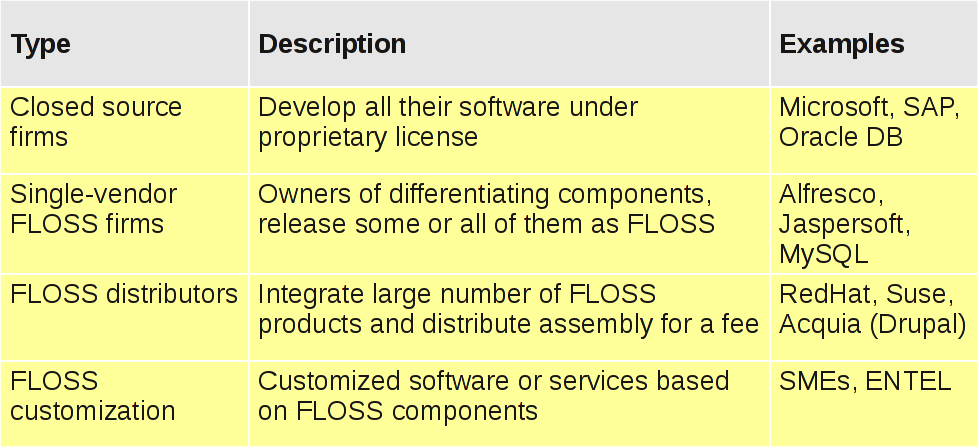
\includegraphics[width=10cm]{figs/sw-development-companies.png}
    \caption{Software companies according to business focus} 
  \end{figure}
\end{center}

\end{frame}

%%%%%%%%%%%%%%%%%%%%%%%%%%%%%%%%%%%%%%%%%%%%%%%%%%%%%%%%%%%%%%%%

\begin{frame}
 \frametitle{IPR strategies}
\begin{itemize}
 \item Two types of ownership strategies in FLOSS:
 \begin{itemize}
  \item \textit{Single-vendor FLOSS}: Only one legal owner of IPR, tipically a software development firm
that exerts itself to maintain its ownership rights.
  \item \textit{Community FLOSS}: This software has either a diffuse group of owners (all code contributors)
or it is owned by a foundation, acting on behalf or all its members
 \end{itemize}
\end{itemize}

\end{frame}

%%%%%%%%%%%%%%%%%%%%%%%%%%%%%%%%%%%%%%%%%%%%%%%%%%%%%%%%%%%%%%%%

\begin{frame}
 \frametitle{FLOSS license strategies}
\begin{itemize}
 \item Two types of strategies related to FLOSS licenses and business models:
 \begin{itemize}
  \item \textit{Reciprocal licenses (\textit{copyleft})}: Force any other company to release their own
products if they use, modify, distribute or integrate FLOSS components under the same license. 
Examples:GPL, AGPL.
  \item \textit{Permissive licences}: Do not force other companies to release their own product under a FLOSS
license if they use, modify, distribute or integrate FLOSS components. Examples: MPL, BSD.
 \end{itemize}
\end{itemize}

\end{frame}

%%%%%%%%%%%%%%%%%%%%%%%%%%%%%%%%%%%%%%%%%%%%%%%%%%%%%%%%%%%%%%%%

\begin{frame}
 \frametitle{Strategic goals}
\begin{itemize}
 \item \textbf{Reduction of development costs}.
 \begin{itemize}
  \item Reuse of available libraries, components, pieces of code, etc. reduce development costs.
 \end{itemize}

 \item \textbf{Maximization of customer exposure}.
  \begin{itemize}
   \item Active promotion of FLOSS project to sell superior product faster and at lower cost (single-vendor).
  \end{itemize}

 \item \textbf{Minimization of competition}.
  \begin{itemize}
   \item FLOSS ecosystems favor strong competition among providers and stakeholders.
   \item Single-vendors and software distributors adopt certain strategies to keep advantage over competitors.
  \end{itemize}

\end{itemize}
\end{frame}

%%%%%%%%%%%%%%%%%%%%%%%%%%%%%%%%%%%%%%%%%%%%%%%%%%%%%%%%%%%%%%%%

\begin{frame}
\frametitle{Control points \& steering mechanisms}

\begin{center}
  \begin{figure}
    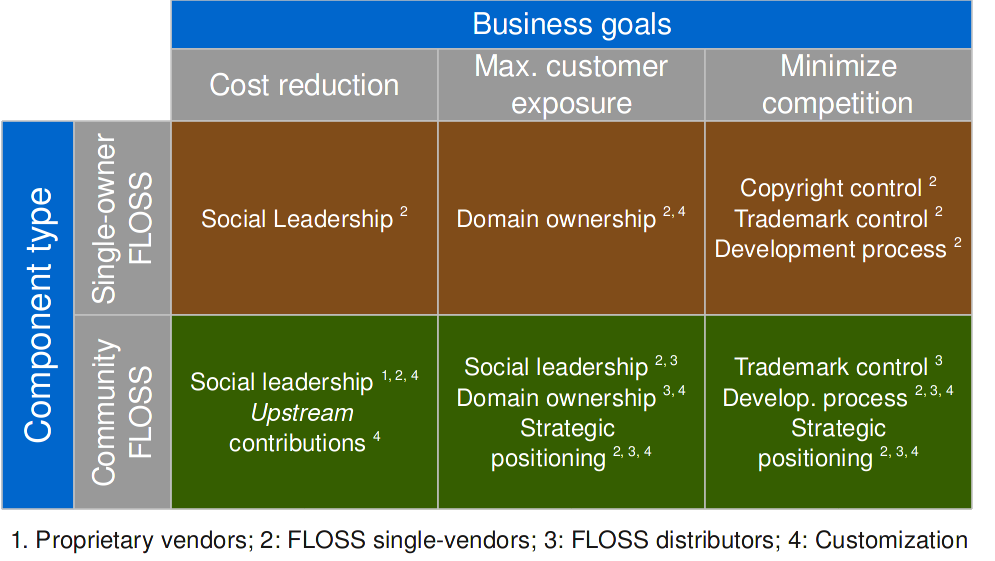
\includegraphics[width=10cm]{figs/control-steering-mechanisms.png}
    \caption{Control points and steering mechanisms in FLOSS business models} 
  \end{figure}
\end{center}

\end{frame}

%%%%%%%%%%%%%%%%%%%%%%%%%%%%%%%%%%%%%%%%%%%%%%%%%%%%%%%%%%%%%%%%

\begin{frame}
 \frametitle{Control points}
\begin{itemize}
 \item Can be enforced thanks to boundary conditions imposed by legal framework:
 \begin{itemize}
  \item \textit{Copyright control}: The company can grant certain rights through FLOSS licenses, but it also
can retain the exclusive copyright ownership. This prevents other third parties to release software under
a different license.
  \item \textit{Trademark control}: Trademarked names and logos deeply embedded in software. It will be costly 
(in terms of bot time and effort) to completely remove them to create \textit{clones}. As well, risk that 
original trademark owner can sue company removing trademarks, under the claim of unfair competition.
  \item \textit{Domain ownership}: Reinforced by trademarks, it contributes to show well-known corporate identity when customers
search for information.
 \end{itemize}
\end{itemize}

\end{frame}

%%%%%%%%%%%%%%%%%%%%%%%%%%%%%%%%%%%%%%%%%%%%%%%%%%%%%%%%%%%%%%%%

\begin{frame}
 \frametitle{Copyright practices}
\begin{itemize}
 \item Typically associated to single-vendor FLOSS firms.
 \begin{itemize}
  \item Requiring copyright transfer for any outside code contribution.
  \item Use reciprocal license to force competitors to release any differentiating improvement
under the same FLOSS lincense.
 \end{itemize}
  \item Copyright ownership enables multiple licensing.
  \item Growing use of licences like AGPL is expected as \textit{cloud} platforms become widespread.
\end{itemize}

\end{frame}

%%%%%%%%%%%%%%%%%%%%%%%%%%%%%%%%%%%%%%%%%%%%%%%%%%%%%%%%%%%%%%%%

\begin{frame}
 \frametitle{Trademark practices}
\begin{itemize}
 \item Important for distributors and single-vendor firms.
 \begin{itemize}
  \item Building a well-known, reliable corporate image to leverage associated products and services.
  \item Original owner will make it as hard as possible to remove any trademarks.
  \item No other competitor can benefit from original owner image.
  \item It fosters: partnerships, certification programs, etc.
 \end{itemize}

\end{itemize}

\end{frame}

%%%%%%%%%%%%%%%%%%%%%%%%%%%%%%%%%%%%%%%%%%%%%%%%%%%%%%%%%%%%%%%%

\begin{frame}
 \frametitle{Domain ownership practices}
\begin{itemize}
 \item Single-vendor firms and distributors use it to protect their own IPR.
 \item Customization companies use it to leverage their added-value and expertise in the market.
 \item Applied in combination with trademarks.
\end{itemize}

\end{frame}

%%%%%%%%%%%%%%%%%%%%%%%%%%%%%%%%%%%%%%%%%%%%%%%%%%%%%%%%%%%%%%%%

\begin{frame}
 \frametitle{Steering mechanisms}
\begin{itemize}
 \item \textit{Social leadership}: Community leadership may contribute
to participate in the definition of community culture, development practices,
evolution plan, partnerships, etc.
 \item \textit{Development process}: Hiring developers, private development process,
delayed distribution.
 \item \textit{Strategic positioning}: Benefit from foundation or alliance to
improve dissemination and public image, keeping advantage over competitors.
\end{itemize}

\end{frame}

%%%%%%%%%%%%%%%%%%%%%%%%%%%%%%%%%%%%%%%%%%%%%%%%%%%%%%%%%%%%%%%%

\begin{frame}
 \frametitle{Social leadership and upstream contributions}
\begin{itemize}
 \item Single-vendor firms employ featured developers, thus influencing the evolution of the FLOSS community
around that product.
 \item Proprietary vendors and customization firms support communities to reduce costs, reusing software components.
 \item Upstream contributions both improve leadership withing the community, and they guarantee compliance with the
source FLOSS components.
\end{itemize}

\end{frame}

%%%%%%%%%%%%%%%%%%%%%%%%%%%%%%%%%%%%%%%%%%%%%%%%%%%%%%%%%%%%%%%%

\begin{frame}
 \frametitle{Development practices}
\begin{itemize}
 \item The company can choose to follow private development process, so all improvements remain hidden from competitors.
 \item It can also decide to delay the release of improvements.
 \item Finally, competitor may only get snapshots of the code base, instead of the full revisioin history of the code repository.
 \item Hide future lines of work from competitors.
\end{itemize}

\end{frame}

%%%%%%%%%%%%%%%%%%%%%%%%%%%%%%%%%%%%%%%%%%%%%%%%%%%%%%%%%%%%%%%%

\begin{frame}
 \frametitle{Strategic positioning}
\begin{itemize}
 \item Usually associated to creation of FLOSS foundation, adding visibility, credibility and
optionally, neutrality.
 \item Example: ASF enforces diversity among developers of new accepted projects.
 \item Legal coverage for distributed copyright ownership.
 \item The foundation may act as a marketing channel to maximize customer exposure.
 \item Single-vendor firms can also leverage strategic baseline communities, to foster innovation in
``low risk'' products, then pick the best contributions to improve enterprise level products.
\end{itemize}

\end{frame}

%%%%%%%%%%%%%%%%%%%%%%%%%%%%%%%%%%%%%%%%%%%%%%%%%%%%%%%%%%%%%%%%

\begin{frame}
 \frametitle{Conclusions}
\begin{itemize}
 \item The business model is just the first step to define the global business strategy of companies.
 \item Around that business model, we need to select adequate control points and steering mechanisms
that will better contribute to ensure its sustainability.
 \item We cannot forget certain conditions:
  \begin{itemize}
   \item Get ready to rapidly react to changes in surrounding market conditions: competitors, partners,
clients, etc.
   \item Understand the advantages of new business relationships: \textit{co-opetition, commoditization, open innovation}, etc.
  \end{itemize}

\end{itemize}

\end{frame}

%%%%%%%%%%%%%%%%%%%%%%%%%%%%%%%%%%%%%%%%%%%%%%%%%%%%%%%%%%%%%%%%

\begin{frame}
 \frametitle{References}
\begin{itemize}
 \item Control points and steering mechanisms in open source software projects.
  \begin{itemize}
  \item \footnotesize{\texttt{http://dirkriehle.com/publications/2010/control-points-}}
    \footnotesize{\texttt{and-steering-mechanisms-in-open-source-software-projects/}}
  \end{itemize}
\end{itemize}

\end{frame}

%%%%%%%%%%%%%%%%%%%%%%%%%%%%%%%%%%%%%%%%%%%%%%%%%%%%%%%%%%%%%%%%
%%

\section{Activity: Rejuvenetion of community controlled FLOSS}

\begin{frame}
\frametitle{Introduction}
\begin{itemize}
  \item Read the following blog post about the evolution of
management stragies in FLOSS-based business models.
  \begin{itemize}
   \item \footnotesize{\texttt{http://blogs.the451group.com/opensource/2009/10/15/}}
   \footnotesize{\texttt{the-rejuvenation-of-community-controlled-open-source/}}
  \end{itemize}
\end{itemize}
\end{frame}

%%%%%%%%%%%%%%%%%%%%%%%%%%%%%%%%%%%%%%%%%%%%%%%%%%%%%%%%%%%%%%%%

\begin{frame}
\frametitle{Questions}
\begin{itemize}
  \item Create groups of 3-4 persons to address the following challenges.
  \item Remember to substantiate your answers with adequate references.
  \begin{itemize}
   \item Find out one example of company identified with each of the 4 stages presented.
   \item What are the main control points and steering mechanisms associated to each stage?
   \item Compare the case of Mozilla Foundation projects and RedHat's Fedora. Explain the
common and different control points and steering mechanisms adopted by each community.
  \end{itemize}
\end{itemize}
\end{frame}

%%%%%%%%%%%%%%%%%%%%%%%%%%%%%%%%%%%%%%%%%%%%%%%%%%%%%%%%%%%%%%%%

%%

\section{Single-vendor vs. Community FLOSS}

\begin{frame}
\frametitle{Introduction}
\begin{itemize}
  \item Two management strategies in FLOSS projects and products:
  \begin{itemize}
   \item \textit{Single-vendor FLOSS}: Copyright owned by a single legal
entity willing to obtain direct revenues from FLOSS product.
   \item \textit{Community FLOSS}: Copyright owned by a community or
neutral legal entity representing the community. Stakeholders does not usually
get direct revenues, but through secondary products and services.
  \end{itemize}

  \end{itemize}
\end{frame}

%%%%%%%%%%%%%%%%%%%%%%%%%%%%%%%%%%%%%%%%%%%%%%%%%%%%%%%%%%%%%%%%

\begin{frame}
\frametitle{Examples}
\begin{itemize}
  \item Single-vendor FLOSS: RedHat, Mozilla software, MySQL.
  \item Community-owned FLOSS: GNOME projects, KDE projects, ASF projects.
\end{itemize}
\end{frame}

%%%%%%%%%%%%%%%%%%%%%%%%%%%%%%%%%%%%%%%%%%%%%%%%%%%%%%%%%%%%%%%%

\begin{frame}
\frametitle{Demand curve in IT solutions}

\begin{center}
  \begin{figure}
    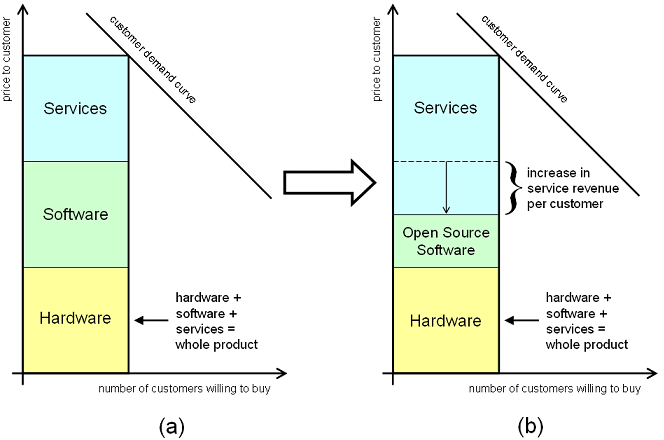
\includegraphics[width=10cm]{figs/it-solutions-demand-curve.png}
    \caption{Taken from The Economic Motivation of Open Source Software: 
Stakeholder Perspectives, by D. Riehle} 
  \end{figure}
\end{center}

\end{frame}

%%%%%%%%%%%%%%%%%%%%%%%%%%%%%%%%%%%%%%%%%%%%%%%%%%%%%%%%%%%%%%%%

\begin{frame}
\frametitle{Business growth in IT markets}

\begin{center}
  \begin{figure}
    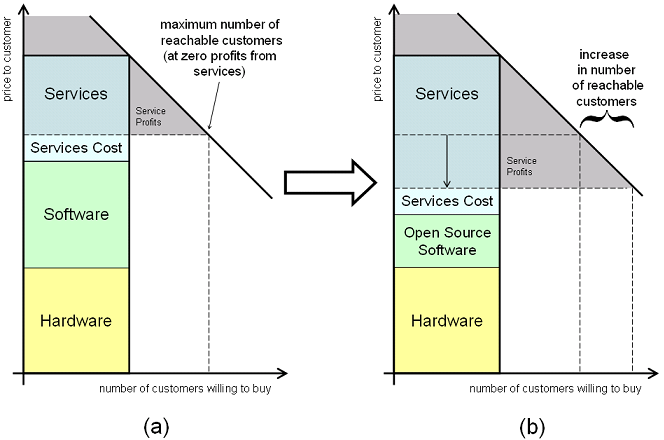
\includegraphics[width=10cm]{figs/business-growth-curve.png}
    \caption{(Taken from The Economic Motivation of Open Source 
Software: Stakeholder Perspectives, by D. Riehle} 
  \end{figure}
\end{center}

\end{frame}

%%%%%%%%%%%%%%%%%%%%%%%%%%%%%%%%%%%%%%%%%%%%%%%%%%%%%%%%%%%%%%%%

\begin{frame}
\frametitle{Single-vendor FLOSS: revenue sources}
\begin{itemize}
  \item Core product.
  \item Whole product.
  \item Operational comfort.
  \item Consulting services.
\end{itemize}
\end{frame}

%%%%%%%%%%%%%%%%%%%%%%%%%%%%%%%%%%%%%%%%%%%%%%%%%%%%%%%%%%%%%%%%

\begin{frame}
\frametitle{Single-vendor also need a community}
\begin{itemize}
  \item FLOSS products without a strong community lead to centralized
development and support problems.
  \item Creating and engaging active communities around single-vendor FLOSS:
  \begin{itemize}
   \item Free use.
   \item No lock-in.
   \item Self support
  \end{itemize}

\end{itemize}
\end{frame}

%%%%%%%%%%%%%%%%%%%%%%%%%%%%%%%%%%%%%%%%%%%%%%%%%%%%%%%%%%%%%%%%

\begin{frame}
\frametitle{Single-vendor: from community to benefits}
\begin{itemize}
  \item Once the single vendor has an active community around its products,
benefits come down the pipe:
  \begin{itemize}
   \item Sales.
   \item Marketing.
   \item Product managment.
   \item Engineering.
   \item Support.
  \end{itemize}

\end{itemize}
\end{frame}

%%%%%%%%%%%%%%%%%%%%%%%%%%%%%%%%%%%%%%%%%%%%%%%%%%%%%%%%%%%%%%%%

\begin{frame}
\frametitle{Example of Single-vendor benefits: sales}
\begin{itemize}
  \item From ``Smoothing the On-ramp to Commercial'', by Larry Augustin.
  \item Single-vendor open source sales funnel (from customers perspective):
  \begin{enumerate}
   \item Download
   \item Install
   \item Use.
   \item Lead.
   \item Prospect
   \item Sale (customer).
  \end{enumerate}

\end{itemize}
\end{frame}

%%%%%%%%%%%%%%%%%%%%%%%%%%%%%%%%%%%%%%%%%%%%%%%%%%%%%%%%%%%%%%%%

\begin{frame}
\frametitle{The role of FLOSS foundations}
\begin{itemize}
  \item Steward of projects under its responsibility.
  \item Financial control, legal coverage and assessment.
  \item Positive added-values: Marketing, public image, negotiations...
  \item The foundation represents the community of developers: 
  \textit{community open source}.
\end{itemize}
\end{frame}

%%%%%%%%%%%%%%%%%%%%%%%%%%%%%%%%%%%%%%%%%%%%%%%%%%%%%%%%%%%%%%%%

\begin{frame}
\frametitle{Market strategy in community FLOSS}

\begin{itemize}
 \item \textit{Law of conservation of attractive profits (Christensen, 2004)}
  \begin{center}
   \begin{quote}
    ``When attractive profits disappear at one stage in the value chain because 
a product becomes modular and commoditized, the opportunity to earn attractive profits 
with proprietary products will usually emerge at an adjacent stage.''
   \end{quote}

  \end{center}

\end{itemize}


\end{frame}

%%%%%%%%%%%%%%%%%%%%%%%%%%%%%%%%%%%%%%%%%%%%%%%%%%%%%%%%%%%%%%%%

\begin{frame}
\frametitle{Market strategy in community FLOSS}
\begin{itemize}
 \item Profits per sale.
\end{itemize}

\begin{center}
  \begin{figure}
    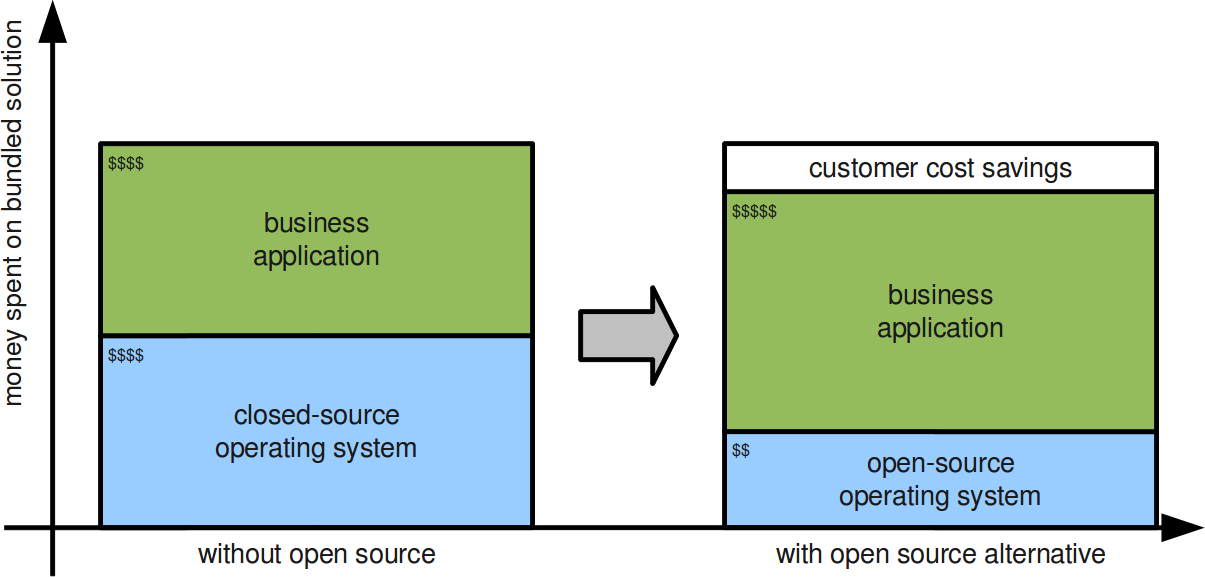
\includegraphics[width=10cm]{figs/floss-vs-closedsw-markets.png}
    \caption{Proprietary software vs. community FLOSS market (from The Economic
Case of Open Source Software Foundations, by D. Riehle)} 
  \end{figure}
\end{center}

\end{frame}

%%%%%%%%%%%%%%%%%%%%%%%%%%%%%%%%%%%%%%%%%%%%%%%%%%%%%%%%%%%%%%%%

\begin{frame}
\frametitle{Market strategy in community FLOSS}

\begin{itemize}
 \item Increased sales in certain market.
\end{itemize}

\begin{center}
  \begin{figure}
    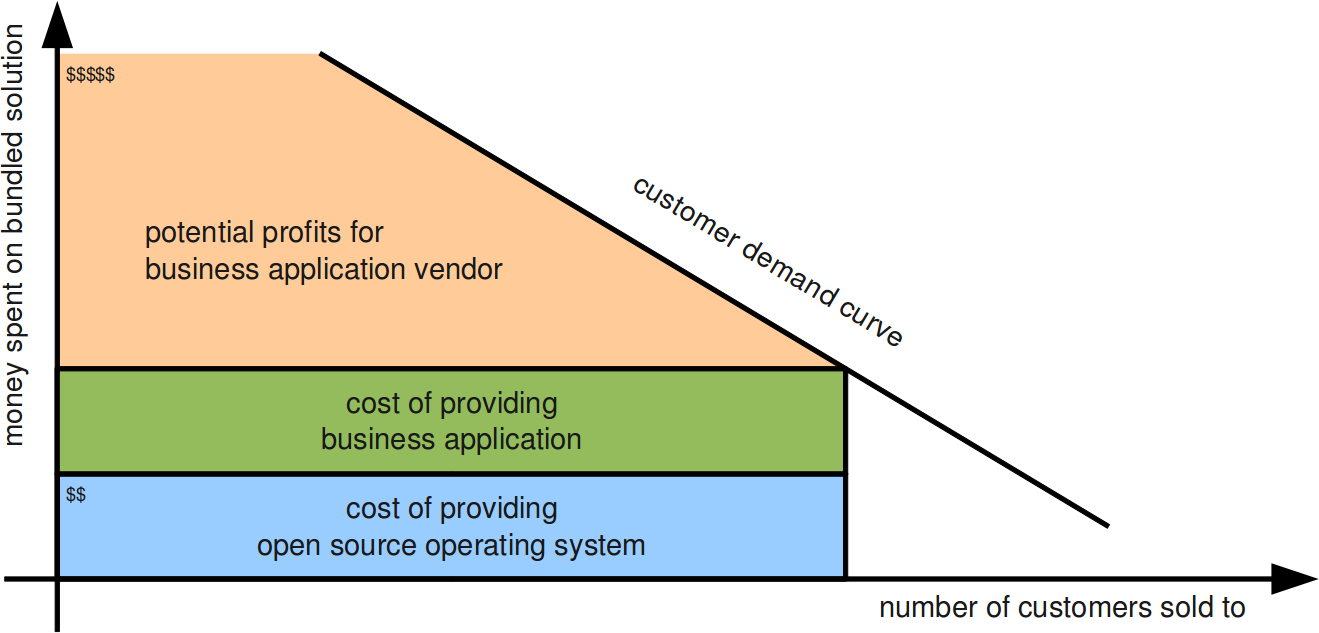
\includegraphics[width=10cm]{figs/customer-demand-curve-floss.png}
    \caption{Customer demand curve in community FLOSS markets (from The Economic
Case of Open Source Software Foundations, by D. Riehle)} 
  \end{figure}
\end{center}

\end{frame}

%%%%%%%%%%%%%%%%%%%%%%%%%%%%%%%%%%%%%%%%%%%%%%%%%%%%%%%%%%%%%%%%

\begin{frame}
\frametitle{Market strategy in community FLOSS}

\begin{itemize}
 \item Larger addressable market.
\end{itemize}

\begin{center}
  \begin{figure}
    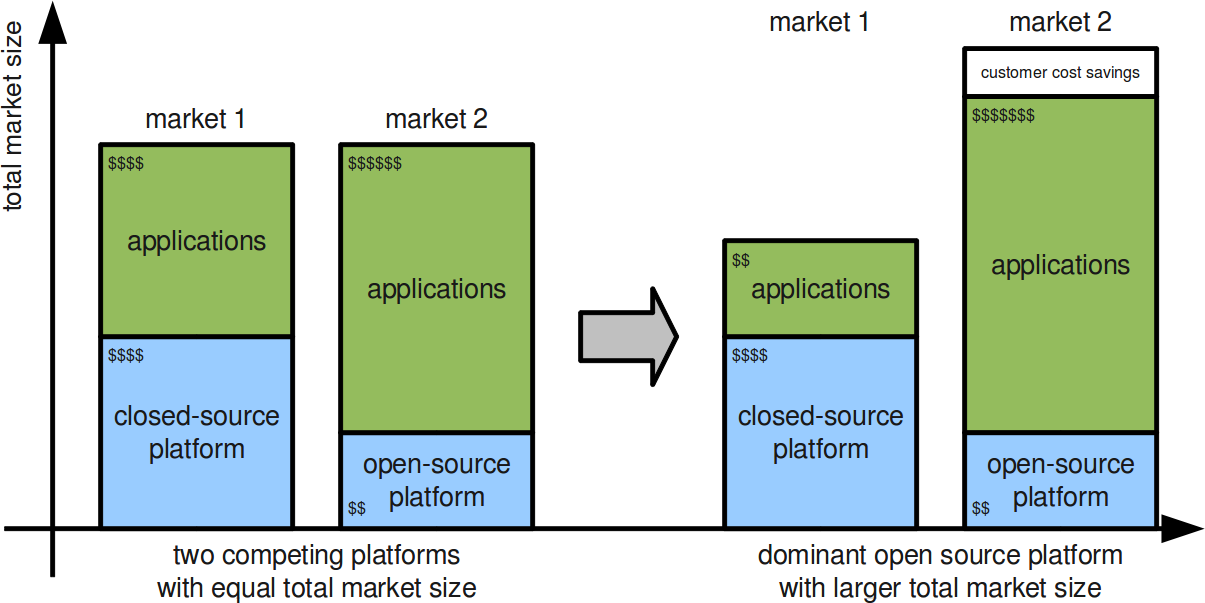
\includegraphics[width=10cm]{figs/growing-floss-platforms-market.png}
    \caption{Larger market size with community FLOSS (from The Economic
Case of Open Source Software Foundations, by D. Riehle)} 
  \end{figure}
\end{center}

\end{frame}

%%%%%%%%%%%%%%%%%%%%%%%%%%%%%%%%%%%%%%%%%%%%%%%%%%%%%%%%%%%%%%%%

\begin{frame}
\frametitle{References}
\begin{itemize}
  \item The Single-Vendor Commercial Open Source Business Model, by D. Riehle.
  \begin{itemize}
   \item \footnotesize{\textit{http://dirkriehle.com/publications/2009/}}
   \footnotetext{\textit{the-commercial-open-source-business-model/}}
  \end{itemize}

  \item The Economic Case for Open Source Foundations, by D. Riehle.
  \begin{itemize}
   \item \footnotesize{\textit{http://dirkriehle.com/publications/2010/}}
   \footnotesize{\textit{the-economic-case-for-open-source-foundations/}}
  \end{itemize}

  \item The Economic Motivation of Open Source Software: Stakeholder Perspectives, by D. Riehle
  \begin{itemize}
   \item \footnotesize{\textit{http://dirkriehle.com/computer-science/research/2007/}}
   \footnotesize{\textit{computer-2007-article.html}}
  \end{itemize}

\end{itemize}
\end{frame}

%%%%%%%%%%%%%%%%%%%%%%%%%%%%%%%%%%%%%%%%%%%%%%%%%%%%%%%%%%%%%%%%

\begin{frame}
\frametitle{References}
\begin{itemize}
  \item The future of open source licensing, by The 451 Group.(Matthew Aslett).
  \begin{itemize}
   \item \footnotesize{\textit{http://blogs.the451group.com/opensource/2010/08/25/}}
    \footnotesize{\textit{the-future-of-open-source-licensing/}}
  \end{itemize}

  \item Estimating savings from OSS code reuse, or: where does the money comes from?, by C. Daffara.
  \begin{itemize}
   \item \footnotesize{\textit{http://carlodaffara.conecta.it/?p=135}}
  \end{itemize}

\end{itemize}
\end{frame}

%%%%%%%%%%%%%%%%%%%%%%%%%%%%%%%%%%%%%%%%%%%%%%%%%%%%%%%%%%%%%%%%

%%

\section{Case study: Oracle acquires Sun Microsystems}

\begin{frame}
\frametitle{Introduction}
\begin{itemize}
  \item The acquisition of Sun Microsystems by Oracle Corp. was one of the
ground-breaking IT news in 2009.
  \item IBM gave up negotiation at \$7 billion.
  \item Oracle bought the company paying \$7.4 billion.
  \end{itemize}
\end{frame}

%%%%%%%%%%%%%%%%%%%%%%%%%%%%%%%%%%%%%%%%%%%%%%%%%%%%%%%%%%%%%%%%

\begin{frame}
\frametitle{3 different cases studies}
\begin{itemize}
  \item The Open Solaris community.
  \item Libre Office from Open Office.
  \item MySQL (antitrust decisions, SkySQL).
\end{itemize}
\end{frame}

%%%%%%%%%%%%%%%%%%%%%%%%%%%%%%%%%%%%%%%%%%%%%%%%%%%%%%%%%%%%%%%%

\begin{frame}
\frametitle{Activity}
\begin{itemize}
  \item Split into 3 groups of comparable size.
  \item Choose one of the 3 topics presented before.
  \item For each topic:
  \begin{enumerate}
   \item Create a chronological list of the featured news and events that
ocurred in that story.
   \item Connect these events with concrete control and steering strageies related
to the new business model exerted by Oracle and community willingness.
   \item Prepare a short presentation to explain your findings to the rest of the
class.
  \end{enumerate}

  \end{itemize}
\end{frame}

%%%%%%%%%%%%%%%%%%%%%%%%%%%%%%%%%%%%%%%%%%%%%%%%%%%%%%%%%%%%%%%%


% Assignments and activities
%%

\section{Assignment: Ten myths about FLOSS business models}


\begin{frame}
\frametitle{Dynamics and goals}

\begin{itemize}
\item Statements based on ``Ten myths about FLOSS business models'', by Carlo Daffara \\
\url{http://www.groklaw.net/articlebasic.php?story=20070828132340846}
\item Each one can be right or wrong (or arguable).
\item Work in groups to give simple answers supporting or rebating the statement.
\item Document your answers with factual arguments, if possible (links, data, etc.).
\end{itemize}
\end{frame}

%%%%%%%%%%%%%%%%%%%%%%%%%%%%%%%%%%%%%%%%%%%%%%%%%%%%%%%%%%%%%%

\begin{frame}
 \frametitle{Statement 1}
 \begin{center}
  \begin{LARGE} FLOSS does not prevent prices from being established for it.  \end{LARGE}
 \end{center}

\end{frame}

%%%%%%%%%%%%%%%%%%%%%%%%%%%%%%%%%%%%%%%%%%%%%%%%%%%%%%%%%%%%%%

\begin{frame}
 \frametitle{Statement 2}
 \begin{center}
  \begin{LARGE} FLOSS licenses aim to suppress any ownership claims, they are hostile to
intellectual property rights.  \end{LARGE}
 \end{center}

\end{frame}

%%%%%%%%%%%%%%%%%%%%%%%%%%%%%%%%%%%%%%%%%%%%%%%%%%%%%%%%%%%%%%

\begin{frame}
 \frametitle{Statement 3}
 \begin{center}
  \begin{LARGE} FLOSS development is mainly driven by ad-hoc altruism and volunteer effort. \end{LARGE}
 \end{center}

\end{frame}

%%%%%%%%%%%%%%%%%%%%%%%%%%%%%%%%%%%%%%%%%%%%%%%%%%%%%%%%%%%%%%

\begin{frame}
 \frametitle{Statement 4}
 \begin{center}
  \begin{LARGE} If I release my software to the FLOSS community, thousands of developers 
will suddenly start working for me, for nothing. \end{LARGE}
 \end{center}

\end{frame}

%%%%%%%%%%%%%%%%%%%%%%%%%%%%%%%%%%%%%%%%%%%%%%%%%%%%%%%%%%%%%%

\begin{frame}
 \frametitle{Statement 5}
 \begin{center}
  \begin{LARGE} Many big companies and firms (even outside software development business) use FLOSS. \end{LARGE}
 \end{center}

\end{frame}

%%%%%%%%%%%%%%%%%%%%%%%%%%%%%%%%%%%%%%%%%%%%%%%%%%%%%%%%%%%%%%

\begin{frame}
 \frametitle{Statement 6}
 \begin{center}
  \begin{LARGE} FLOSS is inherently unreliable, and not very well supported. \end{LARGE}
 \end{center}

\end{frame}

%%%%%%%%%%%%%%%%%%%%%%%%%%%%%%%%%%%%%%%%%%%%%%%%%%%%%%%%%%%%%%

\begin{frame}
 \frametitle{Statement 7}
 \begin{center}
  \begin{LARGE} Private companies contribute to FLOSS, since they can get profit in exchange. \end{LARGE}
 \end{center}

\end{frame}

%%%%%%%%%%%%%%%%%%%%%%%%%%%%%%%%%%%%%%%%%%%%%%%%%%%%%%%%%%%%%%

\begin{frame}
 \frametitle{Statement 8}
 \begin{center}
  \begin{LARGE} Widespread FLOSS projects are invariably funded by large private companies. \end{LARGE}
 \end{center}

\end{frame}

%%%%%%%%%%%%%%%%%%%%%%%%%%%%%%%%%%%%%%%%%%%%%%%%%%%%%%%%%%%%%%

\begin{frame}
 \frametitle{Statement 9}
 \begin{center}
  \begin{LARGE} FLOSS software has achieved to become a market leader in certain sectors.  \end{LARGE}
 \end{center}

\end{frame}

%%%%%%%%%%%%%%%%%%%%%%%%%%%%%%%%%%%%%%%%%%%%%%%%%%%%%%%%%%%%%%

\begin{frame}
 \frametitle{Statement 10}
 \begin{center}
  \begin{LARGE} If a company leading a FLOSS project is acquired, the new owner
can lock the source code and force all its customers to pay for it. \end{LARGE}
 \end{center}

\end{frame}


\section{Assignment: Yockai Benkler on the new open source economics}

\begin{frame}
\frametitle{Dynamics}
\begin{itemize}
\item Some references from video presentation.
\item Possible topics or questions for open debate.
\end{itemize}
\end{frame}

%%%%%%%%%%%%%%%%%%%%%%%%%%%%%%%%%%%%%%%%%%%%%%%%%%%%%%%%%%%%%%

\begin{frame}
 \frametitle{Internet changes information economy}
 \begin{itemize}
  \item 19-20th century: High cost as initial requirement for starting mass circulation of info.
  \item \textit{http://setiathome.berkeley.edu/}
  \item \textit{http://www.chem.ox.ac.uk/cancer/pancreaticcancer.html}
 \end{itemize}


\end{frame}

%%%%%%%%%%%%%%%%%%%%%%%%%%%%%%%%%%%%%%%%%%%%%%%%%%%%%%%%%%%%%%

\begin{frame}
 \frametitle{Needed capital is distributed}
 \begin{itemize}
  \item Apache vs. Microsoft IIS.
  \item \textit{http://beamartian.jpl.nasa.gov/welcome}
  \item \textit{Crowdsourcing}, \textit{wisdom of crowds}...
 \end{itemize}

\end{frame}

%%%%%%%%%%%%%%%%%%%%%%%%%%%%%%%%%%%%%%%%%%%%%%%%%%%%%%%%%%%%%%

\begin{frame}
 \frametitle{New production models, massive distributed communities}
 \begin{itemize}
  \item Google PageRank.
  \item Wikipedia vs. Encarta.
  \item \textit{http://www.crowdspring.com/}
  \item \textit{P2P networks}
 \end{itemize}

\end{frame}

%
% $Id: slides.tex 4228 2006-06-21 21:55:12Z jjamor $
%
%
% Compilar a .pdf con LaTeX (pdflatex)
% Es necesario instalar Beamer (paquete latex-beamer en Debian)
%

%
% Gráficos:
% Los gráficos pueden suministrarse en PNG, JPG, TIF, PDF, MPS
% Los EPS deben convertirse a PDF (usar epstopdf)
%

\documentclass{beamer}
\usetheme{Warsaw}
\usebackgroundtemplate{
\includegraphics[width=\paperwidth]{format/libresoft-bg.png}}
\usepackage[spanish]{babel}
\usepackage[utf8]{inputenc}
\usepackage{graphics}
\usepackage{amssymb} % Simbolos matematicos
\usepackage{url}

%\definecolor{libresoftgreen}{RGB}{162,190,43}
%\definecolor{libresoftblue}{RGB}{0,98,143}

%\setbeamercolor{titlelike}{bg=libresoftgreen}

%% Metadatos del PDF.
\hypersetup{
  pdftitle={Debate open innovation video (C. Leadbeater)},
  pdfauthor={F. Ortega, Jesus M. Gonzalez-Barahona},
  pdfcreator={GSyC/Libresoft},
  pdfproducer=PDFLaTeX,
  pdfsubject={nn},
}
%%


\AtBeginSection[]
{
  \begin{frame}<presentation>
    \frametitle{Index}
    \tableofcontents[current]
  \end{frame}
}


\begin{document}

\title{Debate open innovation video (C. Leadbeater)}
\subtitle{Master on Free Software}
\institute{\\jfelipe@libresoft.es\\
GSyC/Libresoft}
\author{Felipe Ortega, Jesus M. Gonzalez-Barahona}
\date{\today}

\frame{
\maketitle
\begin{center}

\includegraphics[width=6cm]{format/gsyc-urjc}
\end{center}
}


% Si el titulo o el autor se quieren acortar para los pies de p�gina
% se pueden redefinir aqu�:
%\title{Titulo corto}
%\author{Autores abreviado}


%% LICENCIA DE REDISTRIBUCION DE LAS TRANSPAS
\frame{
~
\vspace{4cm}

\begin{flushright}
{\tiny
(cc) 2010 Felipe Ortega, Jesus M. Gonzalez-Barahona. \\
Some rights reserved. This document is distributed under the Creative \\
            Commons Attribution-ShareAlike 3.0 licence, available in \\
            http://creativecommons.org/licenses/by-sa/3.0/

%  Este documento (o uno muy similar) está disponible en \\
%  \url{http://gsyc.escet.urjc.es/~jjamor/}
}
\end{flushright}
}
%%

%%%%%%
%Transpas separadas por \begin{frame}
%%%%%%%%%%%%%%%%%%%%%%%%\end{frame}

%\section{Aim of this exercise}

\begin{frame}
\frametitle{Dynamics}
\begin{itemize}
\item Some references from video presentation.
\item Possible topics or questions for open debate.
\end{itemize}
\end{frame}

%%%%%%%%%%%%%%%%%%%%%%%%%%%%%%%%%%%%%%%%%%%%%%%%%%%%%%%%%%%%%%

\begin{frame}
 \frametitle{Pro-ams/prosumers}
 \begin{itemize}
  \item \textit{http://www.clunkers.net/}
  \item The role of pro-ams and prosumers to drive innovation.
  \item More examples of creativity driven by consumers??
 \end{itemize}


\end{frame}

%%%%%%%%%%%%%%%%%%%%%%%%%%%%%%%%%%%%%%%%%%%%%%%%%%%%%%%%%%%%%%

\begin{frame}
 \frametitle{Creativity an innovation sources}
 \begin{itemize}
  \item Big firms have a built-in tendency to reinforce past positive experiences...
  \item ... but that prevents disruptive innovation to show up.
  \item \textit{http://www2.innocentive.com/}
 \end{itemize}

\end{frame}

%%%%%%%%%%%%%%%%%%%%%%%%%%%%%%%%%%%%%%%%%%%%%%%%%%%%%%%%%%%%%%

\begin{frame}
 \frametitle{Users can be producers}
 \begin{itemize}
  \item \textit{http://en.wikipedia.org/wiki/Shanda}
  \item \textit{http://wikifactcheck.org/}
  \item NewsCorp. \textit{paywall} vs. NYT URL-shortener (social media).
 \end{itemize}

\end{frame}

\end{document}
%%

\section{Activity: identify FLOSS business models}

\begin{frame}
\frametitle{Description}
\begin{itemize}
  \item We present the names of 5 different companies.
  \item For each company, you must find their main business model, according
to the taxonomy from ``FLOSS: a guide for SMEs''.
  \item Some companies might present more than one key business model.
  \item Document your answers as much as possible.
\end{itemize}
\end{frame}

\begin{frame}
 \frametitle{List of companies}
  \begin{enumerate}
   \item BlackDuck.
   \texttt{http://www.blackducksoftware.com/}
   \item Zimbra.
   \texttt{http://www.zimbra.com/}
   \item IBM.
   \texttt{\footnotesize{http://www.ibm.com/developerworks/views/opensource/projects.jsp}}
   \item Jaspersoft.
   \texttt{http://www.jaspersoft.com/}
   \item Funambol.
   \texttt{http://www.funambol.com/}
  \end{enumerate}

\end{frame}



%%

\section{Activity: the open core debate}

\begin{frame}
\frametitle{Introduction}
\begin{itemize}
  \item \textit{Open core} is one of the frequent, yet most controversial
business model strategies around FLOSS.
  \item Open core companies defend their right to maintain proprietary licenses
on strategic features and modules.
  \item FLOSS advocates argue that this approach takes benefit from FLOSS without
giving substantial feedback to communities and projects.
\end{itemize}
\end{frame}

\begin{frame}
 \frametitle{References}
  \begin{enumerate}
   \item Lampitt. ``Open core licensing...''
   \texttt{\footnotesize{http://alampitt.typepad.com/lampitt\_or\_leave\_it/}}
   \texttt{\footnotesize{2008/08/open-core-licen.html}}
   \item Carlo Daffara. ``Relationships between open core, dual licensing and contributions''
   \texttt{\footnotesize{http://carlodaffara.conecta.it/?p=460}}
   \item Simon Phipps. ``Open core is bad for you''.
   \texttt{\footnotesize{http://blogs.computerworlduk.com/simon-says/2010/06/}}
   \texttt{\footnotesize{open-core-is-bad-for-you/}}
   \item OSI. ``A simple declaration about open core''
   \texttt{\footnotesize{http://www.opensource.org/blog/OpenCore}}
  \end{enumerate}

\end{frame}

\begin{frame}
 \frametitle{Questions}
 \begin{itemize}
  \item Find 3 examples of companies following open core strategies.
  \item Could any of these companies switch to a different business model
  and ensure sustainability? How?
  \item Do these companies make any claims on this issue? Summarize
  their arguments.
  \item After learning the arguments from both sides of the story, what is your
  own opinion on this issue?
 \end{itemize}

\end{frame}




%%

\section{Activity: build your FLOSS business model}

\begin{frame}
\frametitle{Description}
\begin{itemize}
  \item Think about an hypothetical start-up company.
  \item Activity based on or revolving around FLOSS.
  \item Create a short business model plan.
\end{itemize}
\end{frame}

\begin{frame}
\frametitle{Organization}

\begin{itemize}
 \item Groups of up to three persons (for discussing the plan)
\item Each student must make her own business project
 \item Name of project.
 \item Goals.
 \item Select license type and strategy.
 \item Briefly detail strategic areas.
\end{itemize}

\end{frame}

\begin{frame}
\frametitle{Economic aspects}

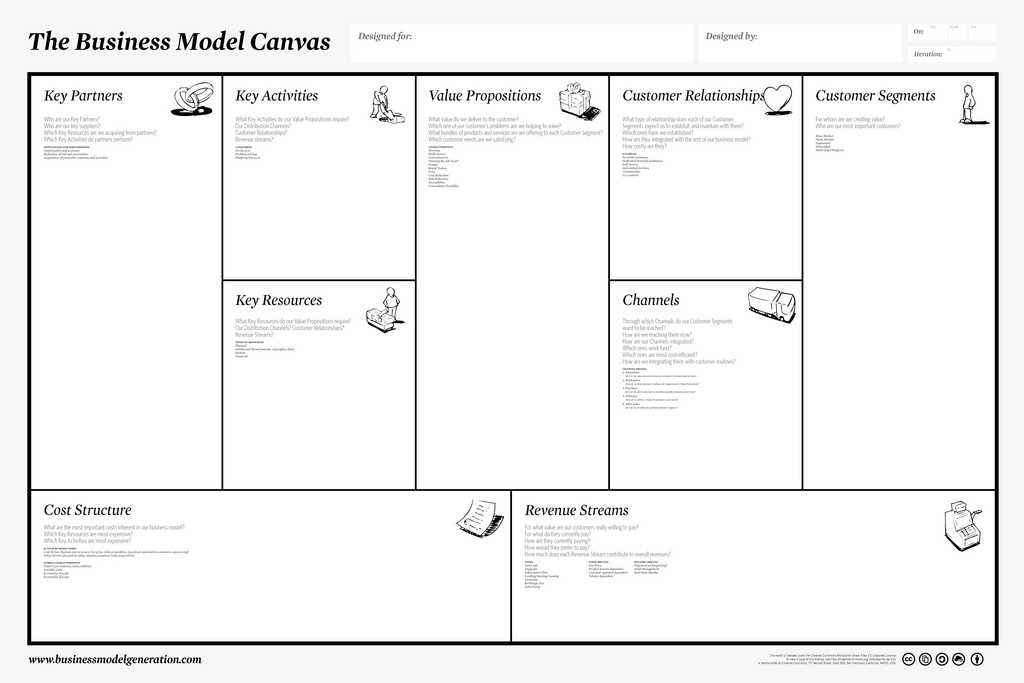
\includegraphics[width=10cm]{figs/business-model-canvas.jpg}

\end{frame}

\begin{frame}
\frametitle{Osterwalder's model}
Suggested order to fill in the canvas.
\begin{itemize}
 \item Clients segments
 \item Value proposal
 \item Channels
 \item Key resources
 \item Cost structure
 \item Revenues streams.
 \item Customer relationships
 \item Key activities
 \item Key partners
\end{itemize}

\end{frame}

\begin{frame}
 \frametitle{References}
\begin{itemize}
 \item \url{http://www.businessmodelalchemist.com/} 
 \item Business Model Generation: A Handbook for Visionaries, Game Changers, and Challengers, A. Osterwalder and Yves Pigneur. Wiley, July 2010.
 \item How to analyze an OSS business model (part 1 to 5).
  \begin{itemize}
   \item \url{http://carlodaffara.conecta.it/?p=372}
   \item \url{http://carlodaffara.conecta.it/?p=379}
   \item \url{http://carlodaffara.conecta.it/?p=387}
   \item \url{http://carlodaffara.conecta.it/?p=395}
   \item \url{http://carlodaffara.conecta.it/?p=413}
  \end{itemize}

\end{itemize}

  
 
 

\end{frame}



\end{document}
